% Send to Mandar (done),Jayesh (done), Aai (done), Baba (done), Arnab (done),Deepak (done) and perhaps Xtof (done), Rahee (done), Ruhi (done), PEB (done), AAO (done), Michael Richards (done), John W (done), Jaydeep K (done), and Grace Gu (done), GR Gogate (done), Chaitanya Bapat (done), Akhil (done), Chinmay (done), Shekhar Divekar (done), Hrishikesh (done), Shilpa Bidwe (done), maybe Prem Andrade (done), Aaron Ashwin (done), Ajay Mishra (done), Vikrant Dhamdhere (done), Sompa (done), Amit Bansal (done), Neelesh Kale (done), Rohit Gondhalekar (done), Piyali (done), Dnyanesh Pawaskar (done).
% Check movies before sending out
\documentclass[12pt]{article}
\usepackage{amsmath}
\usepackage{amsfonts}
\usepackage{cite}
\usepackage{url}
\usepackage{graphicx}
\usepackage{caption}
\usepackage{subcaption}
\usepackage{multirow}
\usepackage{draftwatermark}
\usepackage{pgffor}
% usually hyperref has to be the last package imported
\usepackage{hyperref}
\SetWatermarkText{Draft}
\SetWatermarkScale{10}
%
\newcommand{\beq}{\begin{equation}}
\newcommand{\eeq}{\end{equation}}
\newcommand{\ber}{\begin{eqnarray}}
\newcommand{\eer}{\end{eqnarray}}
\newcommand{\nn}{\nonumber}
\newcommand{\dd}[2]{\frac{d}{d{#2}}{(#1)} }
\newcommand{\pdd}[2]{\frac{\partial{{#1}}}{\partial{#2}}}
% define variables for \mupics command
\newcommand{\nhgscalefactor}{0.24}
\newcommand{\nhgfigheight}{4.0cm}
%\def\nhgvala{true}
%\def\nhgvalb{exxeyy}
%\def\nhgvalc{exxeyynoise}
%\def\nhgvald{eyy}
%\def\nhgvale{eyynoise}
%\def\nhgvalf{uxuy}
%\def\nhgvalg{uy}
%\def\nhgvalh{uynoise}
%\newcommand{\nhgcapmap}[1]{
% https://tex.stackexchange.com/questions/584836/if-statements-in-latex?noredirect=1#comment1470068_584836  
%  \edef\temparg{#1}
%  \ifx\temparg\nhgvala  True  \fi
%  \ifx\temparg\nhgvalb  $\epsilon_{xx}$ \& $\epsilon_{yy}$  \fi
%  \ifx\temparg\nhgvalc  (b) + noise \fi
%  \ifx\temparg\nhgvald  $\epsilon_{yy}$ \fi
%  \ifx\temparg\nhgvale  $\epsilon_{yy}$ + noise\fi
%  \ifx\temparg\nhgvalf  $u_x+u_y$ \fi
%  \ifx\temparg\nhgvalg  $u_y$ \fi
%  \ifx\temparg\nhgvalh  $u_y$ + noise\fi
% }
%
%\newcommand{\nhghfill}[1]{
%  \edef\temparg{#1}
%  \ifx\temparg\nhgvala\hfill\fi
%  \ifx\temparg\nhgvalb\hfill\fi
%  \ifx\temparg\nhgvalc\hfill\fi
%  \ifx\temparg\nhgvald\fi
%  \ifx\temparg\nhgvale\hfill\fi
%  \ifx\temparg\nhgvalf\hfill\fi
%  \ifx\temparg\nhgvalg\hfill\fi
%  \ifx\temparg\nhgvalh\fi
%}
%\newcommand{\nhgmupics}[1]{
%  \foreach \myvar in {\nhgvala,\nhgvalb,\nhgvalc,\nhgvald,\nhgvale,\nhgvalf,\nhgvalg,\nhgvalh}{
%    \begin{subfigure}[b]{\nhgscalefactor\linewidth}
%      \includegraphics[totalheight=\nhgfigheight]{Figures/final/ex#1/mu\myvar.png}
%      \caption{\nhgcapmap{\myvar}}
%    \end{subfigure}
%    \nhghfill{\myvar}
%  }
%}
%
\newcommand{\mupics}[3]{
  % 1
  \hspace{5cm}
  \begin{subfigure}[b]{\nhgscalefactor\linewidth}
    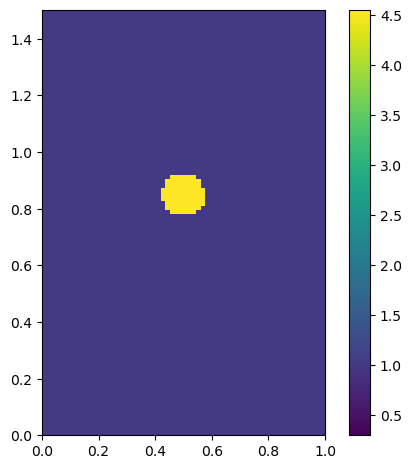
\includegraphics[totalheight=\nhgfigheight]{Figures/final#1/ex#2/mutrue.png}
    \caption{\label{#3a}True}
  \end{subfigure}
  \hspace{5cm}
  \\
  % 2
  \begin{subfigure}[b]{\nhgscalefactor\linewidth}
    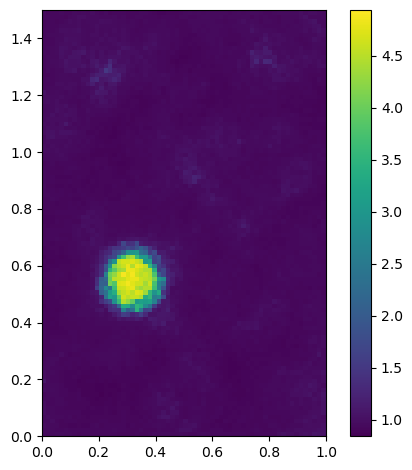
\includegraphics[totalheight=\nhgfigheight]{Figures/final#1/ex#2/muexxeyy.png}
    \caption{\label{#3b}$\epsilon_{xx}$ \& $\epsilon_{yy}$}
  \end{subfigure}
  \hfill
  % 3
  \begin{subfigure}[b]{\nhgscalefactor\linewidth}
    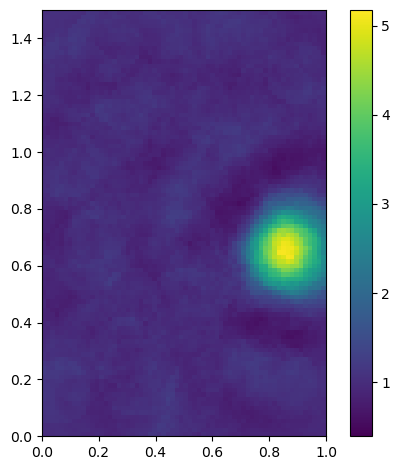
\includegraphics[totalheight=\nhgfigheight]{Figures/final#1/ex#2/muexxeyynoise.png}
    \caption{\label{#3c}(b)+noise}
  \end{subfigure}
  \hfill
  % 4
  \begin{subfigure}[b]{\nhgscalefactor\linewidth}
    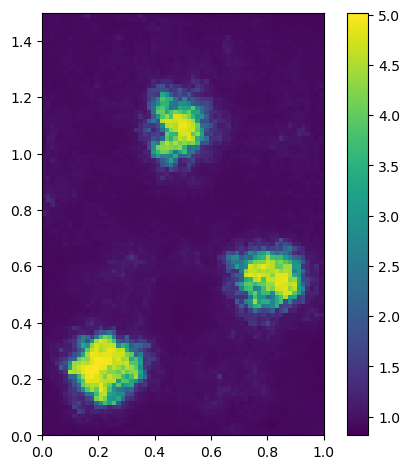
\includegraphics[totalheight=\nhgfigheight]{Figures/final#1/ex#2/mueyy.png}
    \caption{\label{#3d}$\epsilon_{yy}$}
  \end{subfigure}
  \hfill
  % 5
  \begin{subfigure}[b]{\nhgscalefactor\linewidth}
    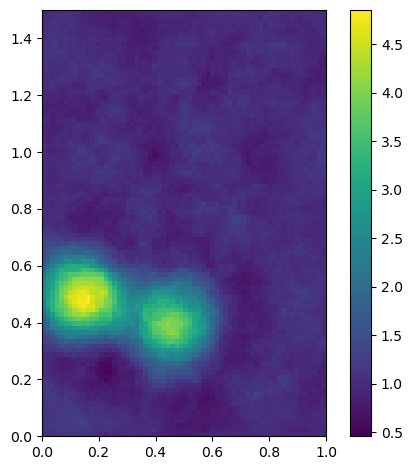
\includegraphics[totalheight=\nhgfigheight]{Figures/final#1/ex#2/mueyynoise.png}
    \caption{\label{#3e}$\epsilon_{yy}$ + noise}
  \end{subfigure}\\
  % 6
  \begin{subfigure}[b]{\nhgscalefactor\linewidth}
    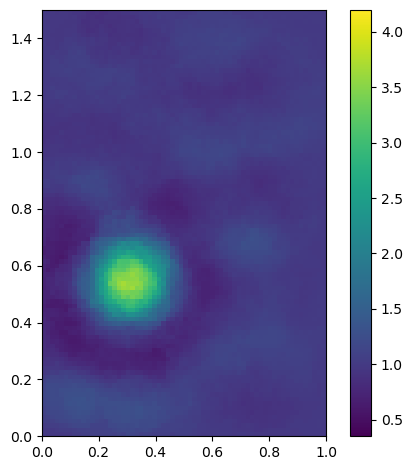
\includegraphics[totalheight=\nhgfigheight]{Figures/final#1/ex#2/muuxuy.png}
    \caption{\label{#3f}$u_{x}$ \& $u_y$}
  \end{subfigure}
  \hfill
  % 7
  \begin{subfigure}[b]{\nhgscalefactor\linewidth}
    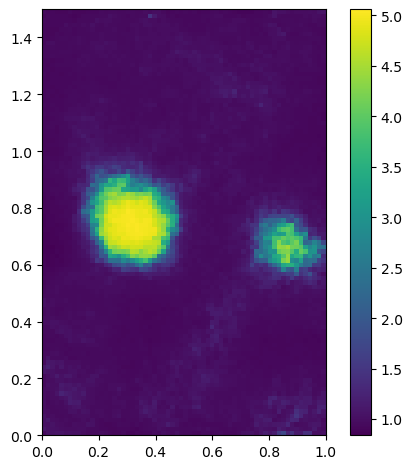
\includegraphics[totalheight=\nhgfigheight]{Figures/final#1/ex#2/muuxuynoise.png}
    \caption{\label{#3g}$u_{x}$ \& $u_y$ + noise}
  \end{subfigure}
  \hfill
  % 8
  \begin{subfigure}[b]{\nhgscalefactor\linewidth}
    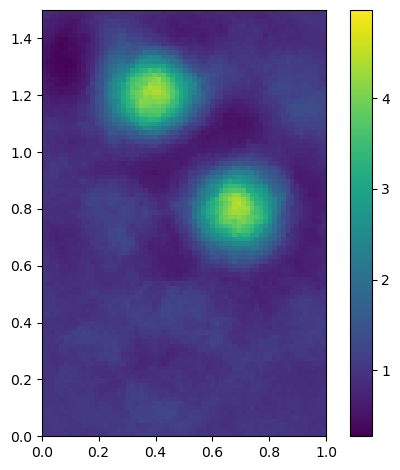
\includegraphics[totalheight=\nhgfigheight]{Figures/final#1/ex#2/muuy.png}
    \caption{\label{#3h}$u_y$}
  \end{subfigure}
  \hfill
  % 9
  \begin{subfigure}[b]{\nhgscalefactor\linewidth}
    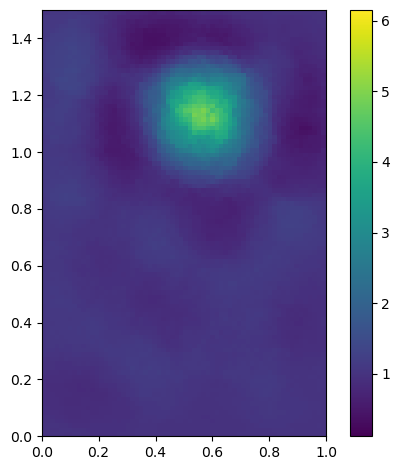
\includegraphics[totalheight=\nhgfigheight]{Figures/final#1/ex#2/muuynoise.png}
    \caption{\label{#3i}$u_y$+noise}
  \end{subfigure}
}
\begin{document}
% bib
\title{Elasticity imaging using a Convolutional Neural Network}
\author{Nachiket Gokhale\footnote{The author is very grateful to Paul Barbone (Professor, Mechanical Engineering, Boston University, Boston, MA, USA.) for patiently answering many questions about finite elements. Conversations with Arnab Majumdar (ArcVisions, Kolkata, India), Michael Richards (Rochester Institute of Technology, Rochester, NY, USA) and Mandar Kulkarni (CGG Veritas, Houston, TX, USA) are gratefully acknowledged and appreciated.}\\gokhalen@gmail.com\\Pune, India.}
\date{\today}
\maketitle
\abstract{We explore the application of a Convolutional Neural Network (CNN) using labeled data (supervised learning) to image the shear modulus field of an almost incompressible elastic medium in plane strain using data which consists of displacement or strains fields (or components thereof). This problem is important in medicine because the shear modulus of suspicious and potentially cancerous growths in soft tissue is elevated by about an order of magnitude as compared to the background of normal tissue. Imaging the shear modulus field therefore can lead to high-contrast medical images. Our prediction problem is as follows: \textit{Given a displacement or strain field (or its components), predict the corresponding shear modulus field}. Our CNN is trained using 2400 training examples consisting of displacement or strain fields (or components thereof) and a corresponding shear modulus field. We present encouraging results which warrant further research and show the promise of this methodology.}
\section{Introduction}
The shear modulus of palpable nodules (which can be thought of as abnormal and potentially cancerous growths in soft tissue) is approximately an order of magnitude higher than the stiffness of the background of normal glandular tissue \cite{paper:sarv1998}. See also Figure (\ref{fig:shearmod}). It follows then, that imaging the shear modulus field of soft tissue results in a high-contrast imaging method because the elevated shear modulus of suspicious growths will stand out clearly against the lower shear modulus of the background of normal tissue. Elasticity Imaging is a broad term that refers to methods which image the shear modulus (or other mechanical properties) of soft tissue in various ways. See \cite{paper:gao1996,paper:parker2010,book:alamgarra2019,bookchap:oberaibarbone2019} for a comprehensive reviews of the field.
%
\begin{figure}[h]
   \centering
    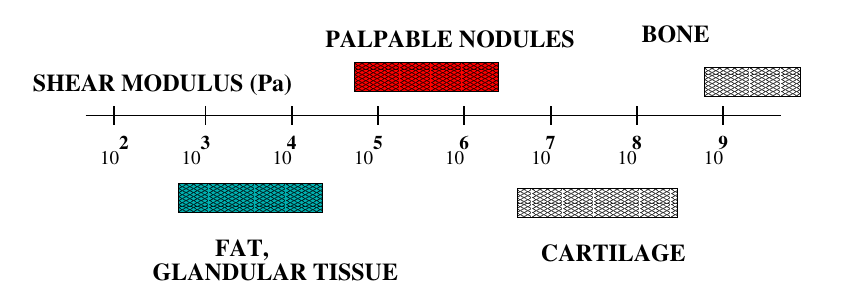
\includegraphics[totalheight=3cm]{Figures/shearmod.png}
  \caption{\label{fig:shearmod} Shear modulii of different types of soft tissue. Adapted from Figure (1) in \cite{paper:sarv1998}.}
\end{figure}
%
\begin{figure}[h]
   \centering
    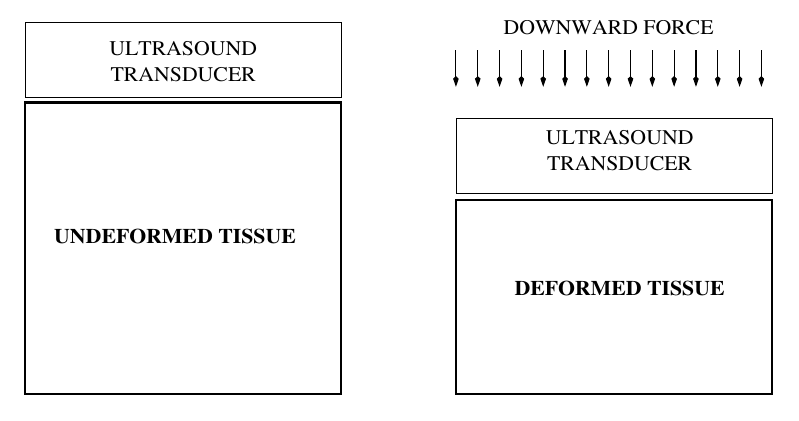
\includegraphics[totalheight=5cm]{Figures/prepostimage.png}
  \caption{\label{fig:prepostimage} Schematic figure showing medical image acquisition when soft tissue is being deformed using ultrasound imaging. The image taken on the left is referred to as the \textit{pre-deformation} image and the image on the right is the \textit{post-deformation image}.}
\end{figure}
%
\subsection{Steps involved in elasticity imaging}
Elasticity Imaging typically consists of the three steps of image acquisition, image registration, inverse problem solution. These steps are discussed in the following sections.
\subsubsection{Image acquisition} Images of soft tissue undergoing deformation due to applied excitation are acquired using various imaging modalities such as ultrasound or magnetic resonance imaging. While time dependent images can be acquired, we shall consider here only two images: a \textit{pre-deformation image} acquired before force is applied and a \textit{post-deformation image} acquired after force is applied. This process is shown in Figure (\ref{fig:prepostimage}) for ultrasound imaging. Also see Figure (2) in \cite{paper:konofagou2004}.
\subsubsection{Image registration} The goal in this step is to find a map which transforms the pre-deformation image into the post-deformation image. For every point in the pre-deformation image we aim to find its location in the post-deformation image. See Figure (\ref{fig:registschematic}). This gives us the \textit{displacement field} between the two images. This displacement field is often referred to as the \textit{measured displacement field}. Differentiating the displacement field with respect to spatial coordinates yields the strain field. If $u_x(x,y)$ and $u_{y}(x,y)$ are the $x$ and $y$ components of the displacement field, then the strain field is given by equation (\ref{eqn:straindef}).
\beq
\label{eqn:straindef}
\epsilon_{xx} = \pdd{u_{x}}{x} \qquad \epsilon_{yy} = \pdd{u_{y}}{y} \qquad \epsilon_{xy} = \frac{1}{2}\Big(\pdd{u_{x}}{y} + \pdd{u_{y}}{x}\Big)
\eeq
See \cite{paper:richards2009,paper:gokhale2004,paper:pellot-barakat2004} for minimization based approaches for computing the displacement field. See \cite{paper:ophir1991,paper:ophir1996,paper:alam1998} and references therein for cross-correlation based approaches. See Figure (\ref{fig:exampdispstrain}) for examples of displacement and strain fields computed using FyPy \cite{misc:fypy}.\\In our work, since we do not have access to medical images we cannot register them to obtain displacement fields. Instead, we generate displacement fields from known shear modulus fields using the finite element method \cite{book:hugheslinear,book:fishbelytschko}.
%
\begin{figure}[h]
  \centering
  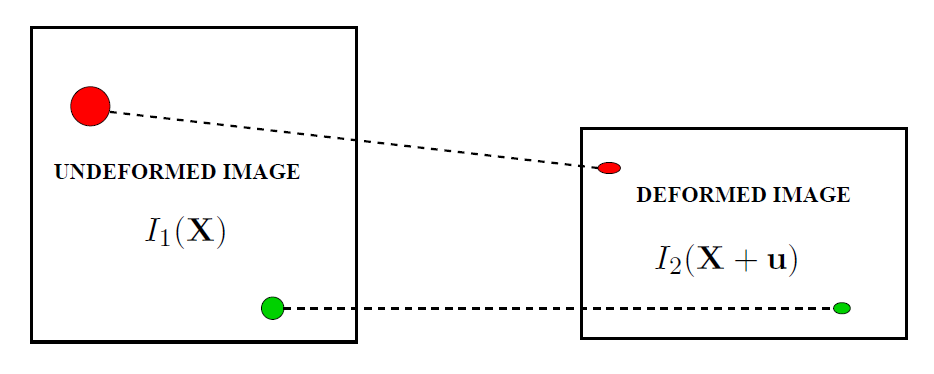
\includegraphics[totalheight=4cm]{Figures/regist.png}
  \caption{\label{fig:registschematic} A schematic figure of image registration. For the red and green points in the pre-deformation image on the left we aim to find their location in the post-deformation image on the right. Doing this for every point in the pre-deformation image yields a displacement field.}
\end{figure}
%
\begin{figure}[h]
  \centering
  %
  \begin{subfigure}[b]{0.25\linewidth}
    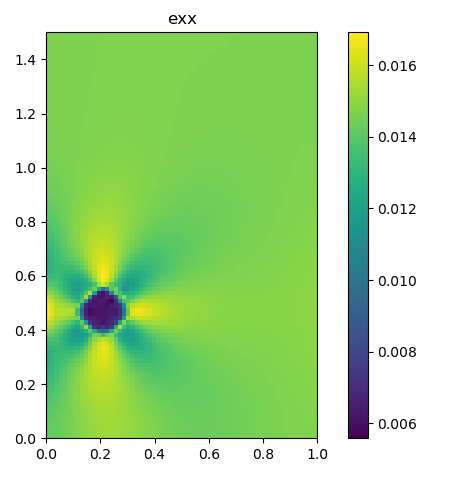
\includegraphics[totalheight=4cm]{Figures/dispstrainfields/exx11_fypy.png}
    \subcaption{$\epsilon_{xx}$}
  \end{subfigure}
  %
  \begin{subfigure}[b]{0.25\linewidth}
    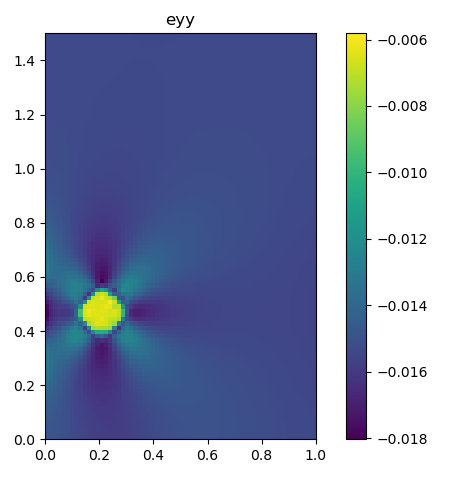
\includegraphics[totalheight=4cm]{Figures/dispstrainfields/eyy11_fypy.png}
    \subcaption{$\epsilon_{yy}$}
  \end{subfigure}
  %
  \begin{subfigure}[b]{0.25\linewidth}
    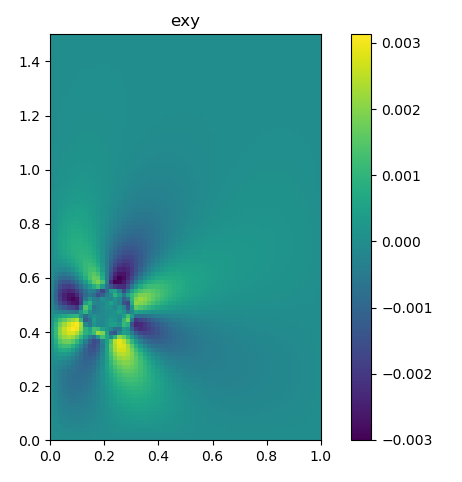
\includegraphics[totalheight=4cm]{Figures/dispstrainfields/exy11_fypy.png}
    \subcaption{$\epsilon_{xy}$}
  \end{subfigure}
  %
  \begin{subfigure}[b]{0.25\linewidth}
    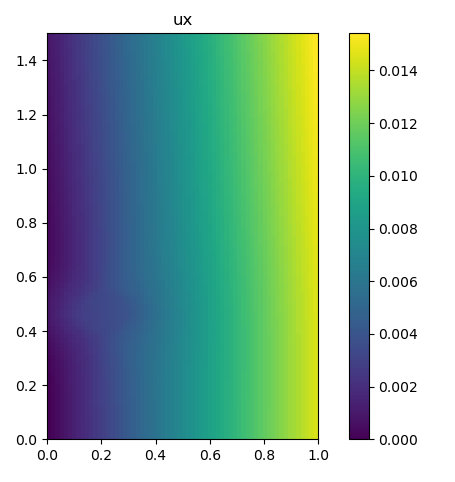
\includegraphics[totalheight=4cm]{Figures/dispstrainfields/ux11_fypy.png}
    \subcaption{$u_{y}$}
  \end{subfigure}
  %
  \begin{subfigure}[b]{0.25\linewidth}
    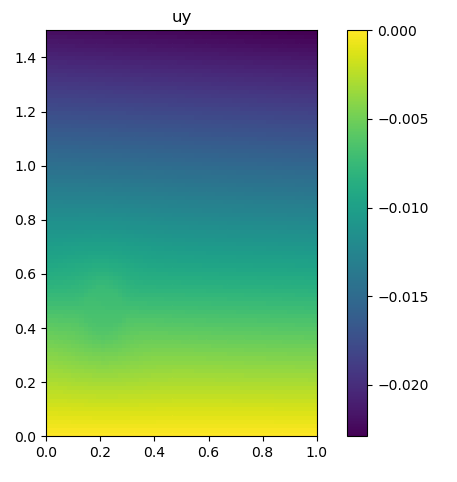
\includegraphics[totalheight=4cm]{Figures/dispstrainfields/uy11_fypy.png}
    \subcaption{$u_{y}$}
  \end{subfigure}
  \caption{\label{fig:exampdispstrain} Examples of displacement and strain fields.}
\end{figure}
\subsubsection{Inverse problem solution} The goal in this step is to infer the spatial distribution of the shear modulus from the displacement field. This is called an \textit{inverse problem} because the classical boundary value problem in linear elasticity (referred to as the \textit{forward problem}) is to determine the displacement field given the shear modulus field, the Poisson's ratio field and suitable boundary conditions. See \cite{book:hugheslinear,book:fishbelytschko} for further details. The approaches for inverse problem solution can be divided into two categories: direct and iterative. These are discussed in the subsequent sections.
\subsubsection{Direct approach} Direct approaches involve solving a single partial differential equation (pde) to obtain the distribution of shear modulus directly: see \cite{paper:raghavan1994,paper:barboneadjwt,paper:albocher}. The coefficients of this pde depend on the measured displacement field. Such approaches are fast and work well when the measured strain field is completely known and has low noise.
\subsubsection{Iterative approach} Iterative approaches \cite{paper:oberai2003,paper:gokhale2008,paper:kalle1996,paper:doyley,paper:goenezen2011} involve guessing a distribution for the shear modulus, solving a linear elasticity forward problem to obtain the predicted displacement field, computing the value and the gradient (and/or Hessian) with respect to the shear modulus of an objective function which consists of a user specified norm of the difference between the predicted displacement field and the measured displacement field, and updating the guessed shear modulus distribution using a suitable optimization procedure such as a modified Newton Raphson scheme as in \cite{paper:doyley} or the BFGS scheme as in \cite{paper:gokhale2008,paper:goenezen2011}. Such approaches are typically slower than direct methods, since the require the solution of approximately $50$ to $100$ forward problems, but have the ability to handle incomplete data and complex nonlinear material models such as hyperelasticity.
\subsubsection{Solving the inverse problem with CNNs}
We believe that solving the inverse problem with CNNs can combine the best characteristics of the direct and iterative approaches. The CNN based approach can yield a quick answer (once time has been spent up front to train the CNN), can accommodate complex constitutive relations, can work with incomplete data (e.g. only a single component of a displacement field) and can work with noisy data. On the other hand, if data which is unlike what the CNN has been trained on is seen, then it is doubtful that the CNN will be able to make correct predictions. Also, CNNs do not predict a perfect result in the absence on noise, unlike traditional direct or iterative methods. On the other hand, it also appears that the performance of CNNs does not degrade as rapidly as direct or iterative methods with increasing noise.
\section{Neural networks and problem setup}
In recent years, neural networks have been applied to various applications such as image classification \cite{paper:hinton2017}, hand written digit recognition \cite{paper:kulkarni2018}, solving differential equations and symbolic integration \cite{misc:lample2019}, solving complex partial differential equations such as the Navier-Stokes equation \cite{misc:anandkumar2020}, self-driving cars \cite{misc:agnihotri2019,misc:nvidiaselfdriving2016}, chaos \cite{paper:pathak2018}, natural language processing \cite{misc:googlenlp}, face recognition \cite{conf:taigman2014} and playing board games such as chess \cite{paper:alphazero}. Several effective Machine Learning frameworks such as Google's TensorFlow \cite{misc:tensorflow} (which we use in this work), Facebook's PyTorch \cite{incollect:pytorch}, Scikit-Learn \cite{paper:scikit-learn} are freely available. See \cite{misc:compdeep} for a complete list. We do not cover the theory of neural networks in this work. The interested reader is referred to \cite{book:aggarwal,book:goodfellow,book:chollet,misc:cs231n,misc:andrewng,misc:udemy} for detailed information about neural networks.
\subsection{Neural networks and elasticity imaging}
Given the success achieved by neural networks on the wide variety of applications cited in the previous section, it is natural to explore the application of neural networks to the inverse problem of elasticity imaging and several recent efforts \cite{paper:pateloberai2019,misc:gu2020,paper:hoeriginsana2016} have done so. In \cite{paper:pateloberai2019}, the authors use a convolutional neural network to classify specimens into elastically heterogeneous or elastically nonlinear. In \cite{paper:hoeriginsana2016}, the authors use a neural network to estimate strains and stress and then calculate elastic parameters. In \cite{misc:gu2020}, the authors use a neural network which predicts elasticity distributions using residual force maps to update the weights of the neural network. \\In contrast, in this work we compute the shear modulus field from the displacement or strain field using a CNN. There are no physical constraints involved in our work. It is purely a mapping problem from the space of displacement or strain fields to the space of the shear modulus fields. The input data for our CNN is a set of strain or displacement fields or components thereof. For each input there is a known corresponding target shear modulus field. Starting from an initial guess of the weights, the CNN predicts shear modulus fields compares them with the target fields to compute the loss function and its gradient. Using the gradient in an appropriate optimization algorithm, the weights are updated. Thus the CNN learns weights for its filters and other parameters. Using this learned information, the CNN is able to predict a shear modulus field from the input data of strain or displacement fields. Figure (\ref{fig:schematic_inv}) shows the mapping of a displacement field to a shear modulus field.\\
It is worth considering if neural networks are really necessary. Consider the following algorithm to solve the elasticity imaging problem.
%
\begin{enumerate}
\item{Let there be $n_{nodes}$ nodes used to discretize the shear modulus and displacement fields.}
\item{Let the shear modulus at each node be allowed to take $n_{\mu}$ discrete values between the minimum shear modulus $\mu_{min}$ and the maximum shear modulus $\mu_{max}$.}
\item{Solve and store displacement fields corresponding to every possible discrete shear modulus field.}
\item{When an unknown displacement field is encountered, find the closest displacement field from step (3) and output the corresponding shear modulus field as the answer.}
\end{enumerate}
The problem with the above algorithm is that the storage required in step (3) is beyond enormous. There are ${n_{\mu}}^{n_{nodes}}$ possible shear modulus fields. This is an enormous number. To see this, take a concrete example: consider $n_{nodes}=1000$ and $n_{\mu}=10$. Then there are $10^{1000}$ possible shear modulus fields. We need an algorithm to search the large search space efficiently. Hence, we need neural networks.
%
\begin{figure}[h]
   \centering
    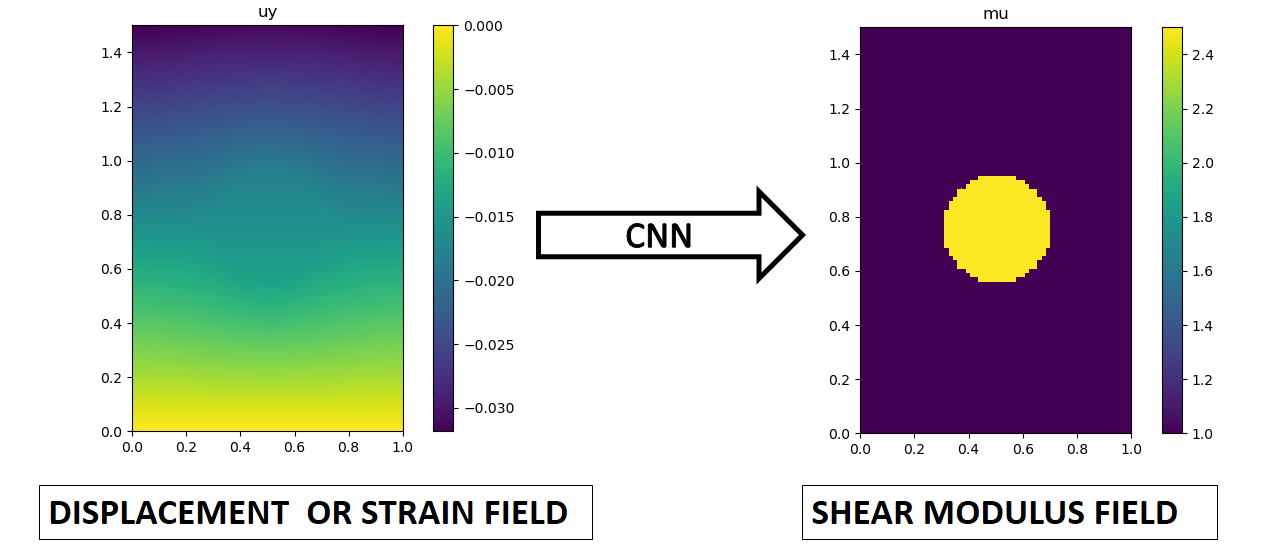
\includegraphics[totalheight=5cm]{Figures/schematic_inv/schematic_inv.png}
  \caption{\label{fig:schematic_inv} Solving the inverse problem using CNNs. The displacement or strain field (or components thereof) are mapped by the CNN into a shear modulus field.}
\end{figure}
%
\subsection{\label{sect:cnnarch} CNN architecture used in this work}
The typical architecture of the CNN we use in this work is shown in Figure (\ref{fig:typical_cnn}) and its parameters are given in Table (\ref{tab:cnnparams}). This CNN was implemented in TensorFlow \cite{misc:tensorflow}. The first dimension '?' represents the number of examples to be processed for training, validation or testing. Thus, the first training example is a three dimensional array and can be accessed using the indices $[0,:,:,:]$ (using Numpy notation) and similarly for the others. The second and third dimensions represent the number of nodes in the $y$ and $x$ direction respectively. The last dimension represents the number of channels in the image. In image-processing the number of channels is typically $3$, one channel each for the three colors red, green and blue (RGB). In our case, the number of channels is the number of components of the displacement or strain field used in our problem. If we use three independent components of the strain field $\epsilon_{xx},\epsilon_{yy},\epsilon_{xy}$ then the number of channels is $3$. If we use only a single component of the strain field, say $\epsilon_{xx}$ only, then the number of channels is $1$. Table (\ref{tab:cnnone:io}) gives the number of channels for each CNN trained. The \textit{loss function} is \textit{mean squared error} and the optimizer is \textit{Adam} with default settings. No regularization is used.  Each CNN has approximately $3.35$ million trainable parameters. After training, the model with the best validation loss is chosen to make predictions.\\The softplus activation function in equation (\ref{eqn:softplus}) and the twisted tanh activation function in equation (\ref{eqn:twisttanh}) are considered in this work. The predictions made using the softplus only respect the basic positivity constraint on the shear modulus i.e. $\mu(x) > 0$. When using the softplus activation, the training shear modulus data is not normalized and while using the twisted tanh function the training shear modulus data is normalized to the range $(-1,1)$.\\ It is seen that the CNNs using the softplus activation tend to predict regions of low shear modulus surround the inclusions. Therefore we seek to restrict the range of the shear modulus predicted by the CNN to within known limits $[\mu_{back},\mu_{max}]$. $\mu_{back}$ is the background shear modulus and this is typically the lowest shear modulus in the problem. $\mu_{max}$ is the maximum shear modulus in the problem. One can simply do this by thresholding: just apply \textit{min} and \textit{max} functions to the shear modulus images produced by using the softplus activation function and post-process the result. But this is unsatisfying because it does not restrict the output of the CNN. \\We considered restricting the output of the CNN to a specified range by first applying a suitable scaling to change the range of the output variable from $[\mu_{back},\mu_{max}]$ to $(0,1)$ or $(-1,1)$ as appropriate. We then considered the use of activation functions given in equations (\ref{eqn:sigmoid},\ref{eqn:tanh},\ref{eqn:softplusmin}) whose range is restricted to $(0,1),(-1,1)$ and $(0,1)$. As noted in \cite{bookchap:lecun98b} we observed that with the activation functions given in equations (\ref{eqn:sigmoid},\ref{eqn:tanh},\ref{eqn:softplusmin}) the weights and therefore loss function become stuck because the derivatives of equations (\ref{eqn:sigmoid},\ref{eqn:tanh},\ref{eqn:softplusmin}) become very close to zero for values sufficiently away from zero. However, we again observe as noted in \cite{bookchap:lecun98b}, that the addition of a \textit{twisting term} ($0.01x$) to the $\tanh(x)$ function makes the derivative non-zero and training of the CNN occurs. While the twisting term changes the range of $\tanh$ from $(-1,1)$ to $(-\infty,+\infty)$, it is observed that in practice the predictions are approximately restricted to the range $[\mu_{back},\mu_{max}]$. We also observe that using the twisted tanh activation results in shear modulus images in which a region of low shear modulus is not seen next to inclusions.
\begin{subequations}
\ber
\text{softplus}\qquad f(x) &=& \ln(1+\exp(x)) \label{eqn:softplus}\\
\text{sigmoid}\qquad f(x) &=& \frac{1}{1+\exp(-x)}\label{eqn:sigmoid}\\
\text{tanh} \qquad f(x) &=& \tanh(x) \label{eqn:tanh}\\
\text{softplusmin} \qquad f(x) &=& \min(\ln(1+\exp(x)),1.0)\label{eqn:softplusmin} \\
\text{twisted tanh} \qquad f(x) &=& \tanh(x) + 0.01x  \label{eqn:twisttanh}
\eer
\end{subequations}
%
\begin{figure}[h]
  \centering
  %
  \begin{subfigure}[b]{0.45\linewidth}
    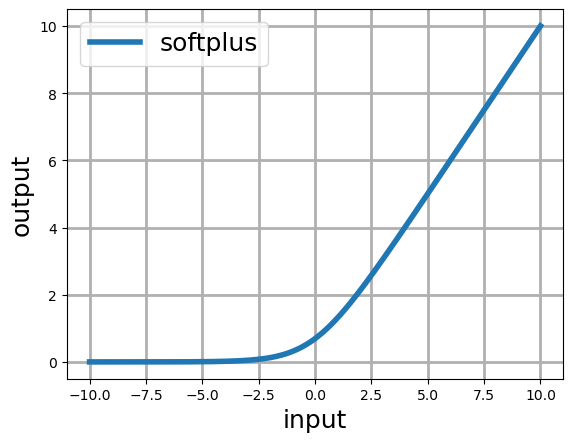
\includegraphics[totalheight=4cm]{Figures/scripts/softplus.png}
    \caption{softplus}
  \end{subfigure}
  %
  \begin{subfigure}[b]{0.45\linewidth}
    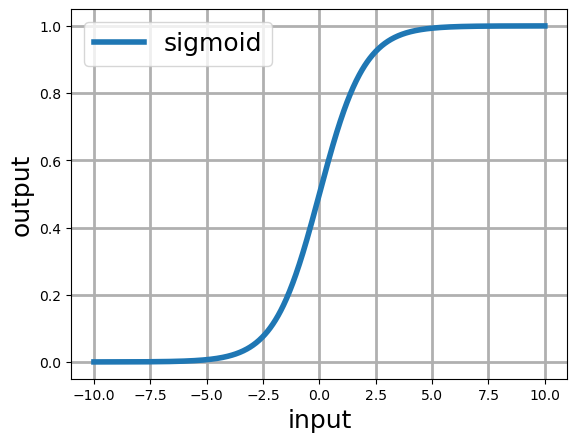
\includegraphics[totalheight=4cm]{Figures/scripts/sigmoid.png}
    \caption{sigmoid}
  \end{subfigure}
  %
  \begin{subfigure}[b]{0.45\linewidth}
    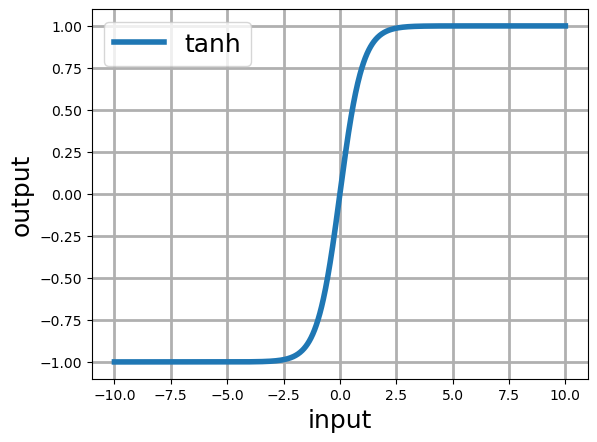
\includegraphics[totalheight=4cm]{Figures/scripts/tanh.png}
    \caption{tanh}
  \end{subfigure}
  %
  \begin{subfigure}[b]{0.45\linewidth}
    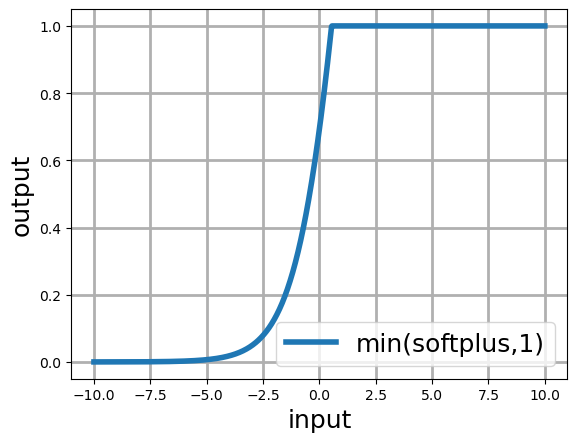
\includegraphics[totalheight=4cm]{Figures/scripts/minsoftplus.png}
    \caption{softplusmin}
  \end{subfigure}
  %
  \begin{subfigure}[b]{0.45\linewidth}
    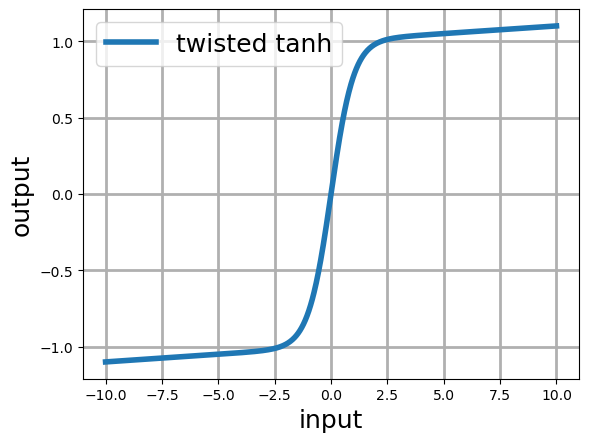
\includegraphics[totalheight=4cm]{Figures/scripts/twistedtanh.png}
    \caption{twisted tanh}
  \end{subfigure}
  %
\caption{\label{fig:activations} Activations functions for equations (\ref{eqn:softplus}-\ref{eqn:twisttanh}).}
\end{figure}
%
\begin{table}
  \centering
 \begin{tabular}{|c|c|}
   \hline
   CNN Layer & Specifications \\
   \hline
   conv2d    & $32$ filters, kernel size $3$, activation is \textit{relu}, no regularization\\
   \hline
   max\_pooling2d: & pool size $2$, strides $2$\\
   \hline
   conv2d\_1 & $64$ filters, kernel size $3$, activation is \textit{relu}, no regularization\\
   \hline
   max\_pooling2d\_1: & pool size $2$, strides $2$\\
   \hline
   flatten & -\\
   \hline
   dense   & $128$ units, activation \textit{relu}, no regularization\\
   \hline
   dense\_1 & $nnodex*nnodey$ units, activation softplus, no regularization\\
   \hline
 \end{tabular}
 \caption{\label{tab:cnnparams} Parameters for the CNN shown in Figure (\ref{fig:typical_cnn}).}
\end{table}
%
\begin{figure}[h] 
   \centering
    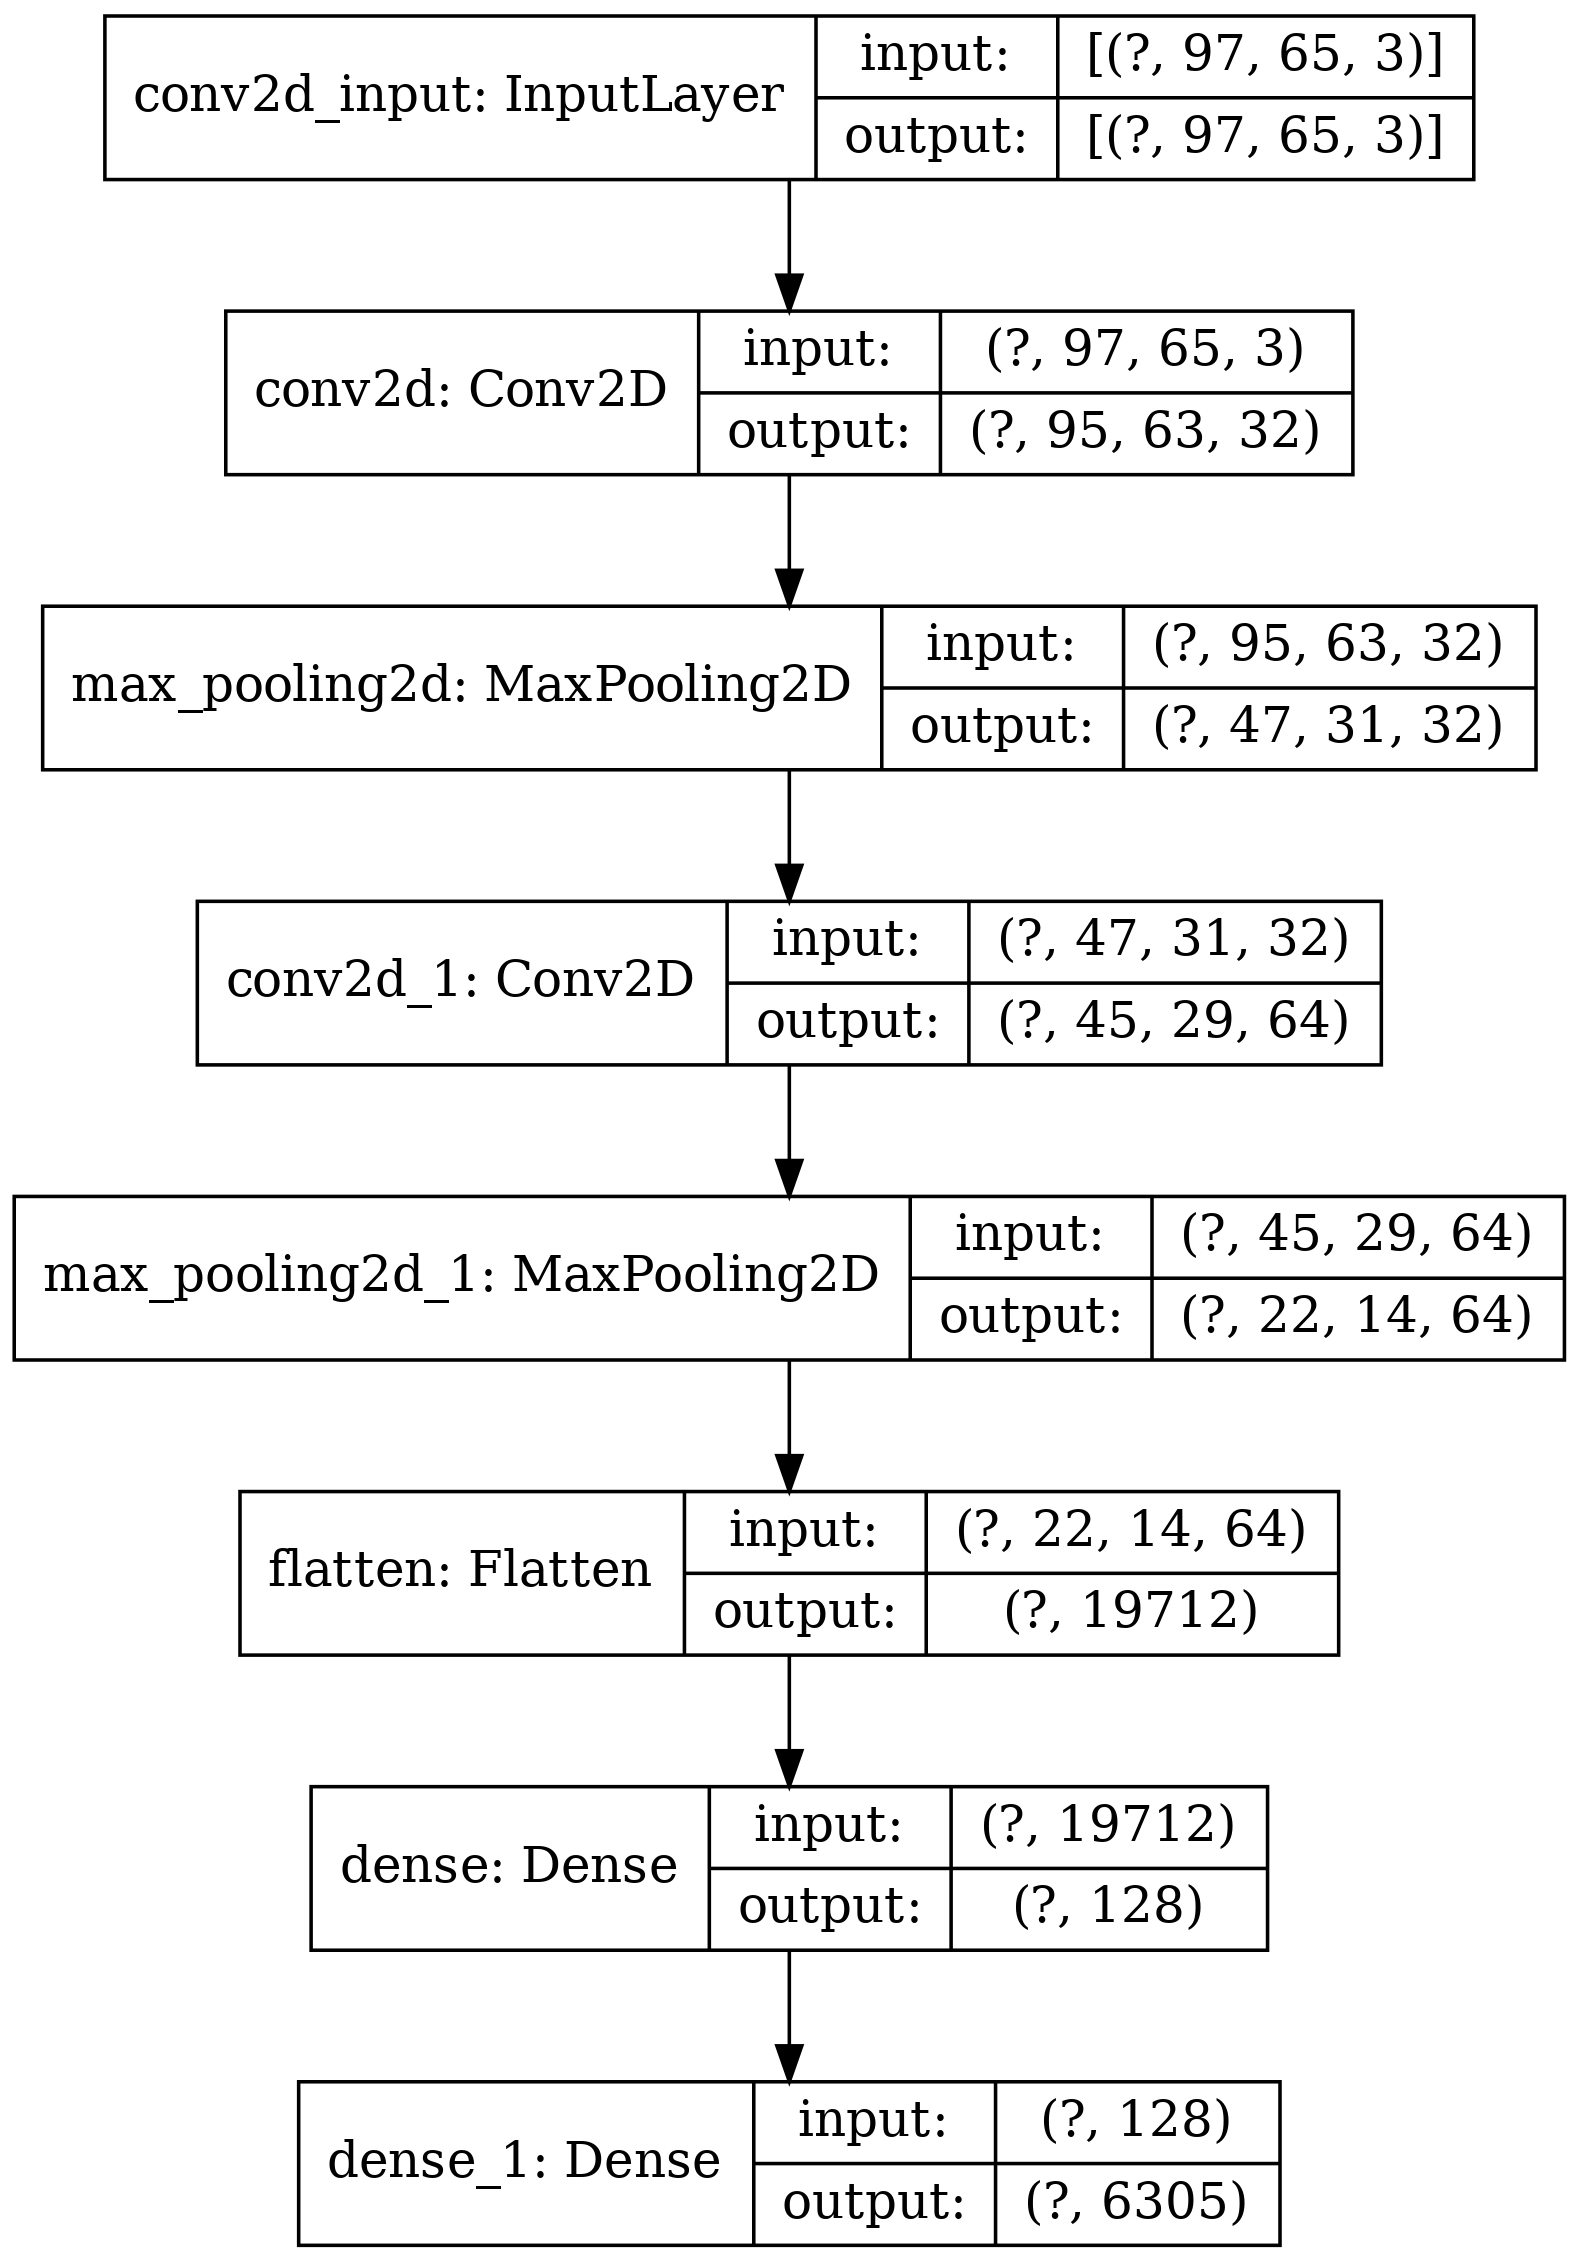
\includegraphics[totalheight=9cm]{Figures/typical_cnn.png}
    \caption{\label{fig:typical_cnn}Typical CNN architecture used in this work. This architecture is essentially the same the one used in the Deep Learning example in \cite{misc:udemy} in which it was used to classify images into two categories: 'cat' or 'dog'.}
\end{figure}
%
%
\subsection{\label{sect:probsetup}Problem setup}
The displacement or strain field data required for the CNN is generated using a linear finite element solver named FyPy (\textbf{Fy}nite Elements in \textbf{Py}thon) \cite{misc:fypy}. The reader is referred to \cite{book:hugheslinear,book:fishbelytschko} for details about the boundary value problem of linear elasticity and its solution using finite elements. Both displacements and material properties are interpolated bilinearly. The problem geometry is shown in Figure (\ref{fig:bc}). Plane strain is assumed. The length (in the $x$ direction) is $1.0$ unit. The breadth (in the $y$ direction) is 1.5 units. Both degrees of freedom are constrained at the pin and only the $y$ degree of freedom is constrained at the roller. The background shear modulus is $\mu_{back}=1.0$ unit. The Poisson's ratio is a constant and is set to $0.49$. Selective reduced integration is used to avoid mesh locking because the Poisson's ratio of $0.49$ renders the medium almost incompressible. There is exactly one inclusion in the domain and its shear modulus is a constant and is a random number ranging from $\mu_{min}=2.0$ to $\mu_{max}=5.0$. There are no homogeneous examples. The radius of the inclusion is a random number ranging from $0.05$ to $0.15$.\\
$4000$ displacement and strain images are generated and are split into $2400$ training examples, $800$ validation examples and $800$ test examples. Each displacement or strain component is scaled by finding the maximum of its absolute value over the training data set and then dividing the component by it. When noisy data is used we add noise in the strain or displacement data such that the signal to noise ratio (SNR) is 40dB using equation (\ref{eqn:snr}). The data is made noisy by element wise multiplication of the strain or displacement data with a matrix containing random numbers in the interval $(1-\epsilon,1+\epsilon)$ where $\epsilon$ is chosen appropriately to yield $\approx$ 40dB noise. We note that noisy data is generated for each run. We do not save noisy test examples for once and for all. Referring to Table (\ref{tab:cnnone:io}), this means, that the noise in $\epsilon_{yy}$ in line 1 is different from the noise in $\epsilon_{yy}$ in line 2. We do not train CNNs with noisy data. Training of the CNN is always carried out on noiseless data and noisy data is given to the CNN as input. 
\begin{equation}
  \label{eqn:snr}
  SNR_{dB} = 20\log_{10}\Big(\frac{\|signal\|_{L^2}}{\|noise\|_{L^2}}\Big)
\end{equation}
The norm $\|\cdot\|_{L^2}$ in the above equation is a discrete $L^2$ norm. 
% Noise details
%
\begin{figure}[h] 
   \centering
    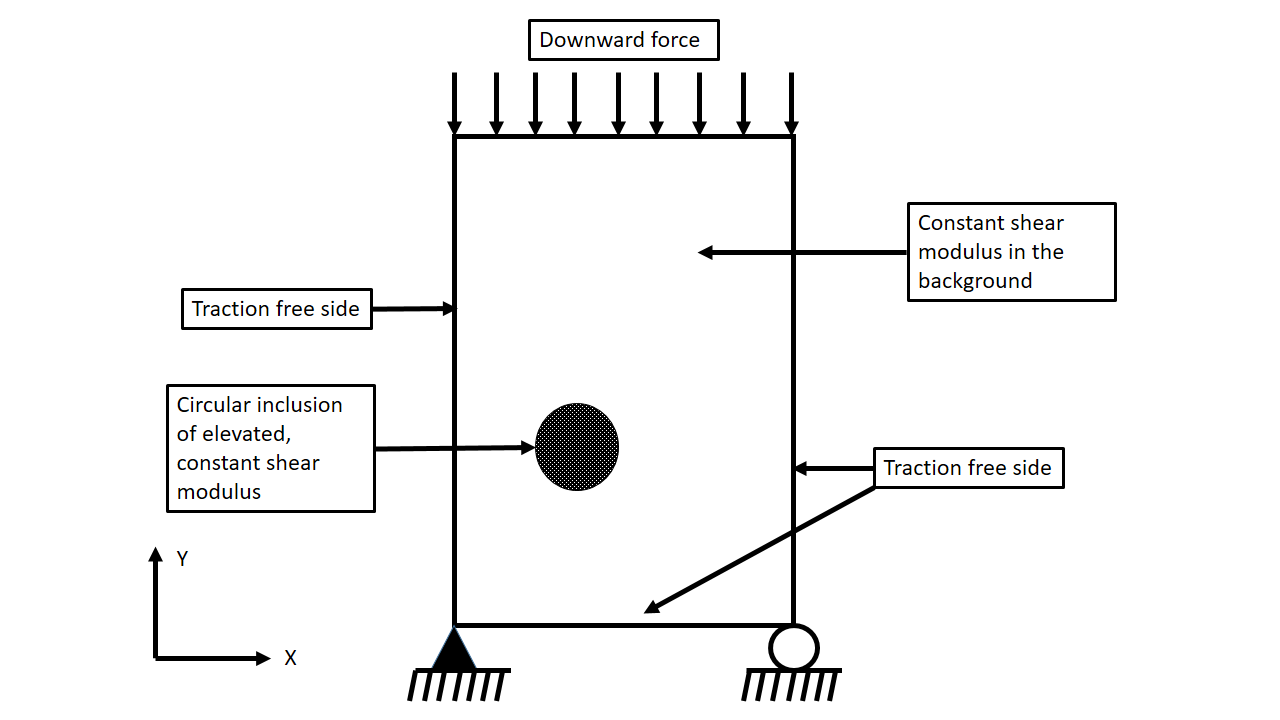
\includegraphics[totalheight=9cm]{Figures/bc.png}
  \caption{\label{fig:bc}Boundary conditions and material properties used in this work. }
\end{figure}
%
\section{\label{sect:oneinc}Imaging one inclusion}
We apply the CNN described in Section (\ref{sect:cnnarch}) to predict the shear modulus field when only one inclusion is present. The data is generated as described in Section (\ref{sect:probsetup}). Eight CNNs are trained. See Table (\ref{tab:cnnone:io}) where the training data and prediction data for each CNN is specified. For example, the first entry in Table (\ref{tab:cnnone:io}) should be interpreted as: CNN $\epsilon_{xx}$ \& $\epsilon_{yy}$ and CNNc $\epsilon_{xx}$ \& $\epsilon_{yy}$ are trained on both components of a noiseless strain field (given in column 2) and are used to make predictions using both components of the strain field, with and without noise (given in column 3). Since two components of the strain field are used to train and make predictions the number of channels is $3$.\\The CNNs using the softplus activation function (equation \ref{eqn:softplus}) to make predictions are:
\begin{enumerate}
\item{CNN $\epsilon_{xx}$ \& $\epsilon_{yy}$}
\item{CNN $\epsilon_{yy}$}
\item{CNN $u_x$ \& $u_y$}
\item{CNN $u_y$}
\end{enumerate}
The CNNs using the twisted tanh (\ref{eqn:twisttanh}) function to make predictions are:
\begin{enumerate}
\item{CNNc $\epsilon_{xx}$ \& $\epsilon_{yy}$}
\item{CNNc $\epsilon_{yy}$}
\item{CNNc $u_x$ \& $u_y$}
\item{CNNc $u_y$}
\end{enumerate}
The additional 'c' at the end of 'CNNc' denotes 'constrained'. We refer to the CNNs using the twisted tanh activation function as constrained because their output is restricted to approximately the interval:$(\mu_{back},\mu_{max})$. See Section (\ref{sect:cnnarch}) for a detailed discussion. \\
The training and loss curves for the CNNs are shown in Figures (\ref{fig:oneinc:trainexxeyy}-\ref{fig:oneinctanh:trainuy}). The predictions of the various CNNs are shown in Figures (\ref{fig:oneinc:1}-\ref{fig:oneinctanh:16}). The results for the CNNs using softplus activation and the CNNs using the twisted tanh activation are presented alternately. All figures on the same page are on the same color scale. The subcaptions of the figures are explained in Table (\ref{tab:subcap}).\\
The conclusions that can be drawn from Figures (\ref{fig:oneinc:1}-\ref{fig:oneinctanh:16}) are:
\begin{enumerate}
\item{The location of the inclusion is predicted accurately.}
\item{Generally speaking, the shear modulus of small inclusions is under-predicted for CNNs. See Figures (\ref{fig:oneinc:1},\ref{fig:oneinc:3},\ref{fig:oneinc:6},\ref{fig:oneinc:8}).}
\item{The shear modulus of large inclusions is correct on average. The discontinuities in the true shear modulus field are not predicted accurately. Instead a smooth field is predicted. The CNNs using the twisted tanh activation do better in predicting discontinuities.}
\item{It is observed that the CNNs using the softplus activation predict a region of low shear modulus next to a region of high shear modulus. See Figures (\ref{fig:oneinc:1},\ref{fig:oneinc:2},\ref{fig:oneinc:3},\ref{fig:oneinc:3}).}
\end{enumerate}
%
\begin{center}
\begin{table}
  \centering
  \begin{tabular}{|p{3cm}|p{2cm}|p{3cm}|p{1.5cm}|}
    \hline
    CNN Name & Training data (noiseless) & Prediction data & Channels\\
    \hline
    CNN $\epsilon_{xx}$ \& $\epsilon_{yy}$ &  $\epsilon_{xx}$ \& $\epsilon_{yy}$ & $\epsilon_{xx}$ \& $\epsilon_{yy}$ & 2\\
    CNNc $\epsilon_{xx}$ \& $\epsilon_{yy}$ &  & $\epsilon_{xx}$ \& $\epsilon_{yy}$ + noise & \\
    \hline
    CNN $\epsilon_{yy}$ & $\epsilon_{yy}$ & $\epsilon_{yy}$ & 1\\
    CNNc $\epsilon_{yy}$ &  & $\epsilon_{yy}$ + noise & \\
    \hline
    CNN $u_x$ \& $u_y$ & $u_x$ \& $u_y$ & $u_x$ \& $u_y$ & 2\\
    CNNc $u_x$ \& $u_y$&  & $u_x$ \& $u_y$ + noise & \\    
    \hline
    CNN $u_y$  & $u_y$ & $u_y$ & 1\\
    CNNc $u_y$ &  & $u_y$ + noise & \\
    \hline
  \end{tabular}
  \caption{\label{tab:cnnone:io} Listing of CNNs trained, their training, prediction data and number of channels. CNN $\epsilon_{xx}$ \& $\epsilon_{yy}$, CNN $\epsilon_{yy}$, CNN $u_x$  and CNN $u_y$ use the softplus activation function for the output layer. CNNc $\epsilon_{xx}$ \& $\epsilon_{yy}$, CNNc $\epsilon_{yy}$, CNNc $u_x$  and CNNc $u_y$ use the twisted tanh activation function for the output layer.}
\end{table}
\end{center}
%
\begin{table}
  \centering
   \begin{tabular}{cp{8cm}}
    \hline
    \multicolumn{1}{|c|}{Subcaption} & \multicolumn{1}{c|}{Meaning}\\
    \hline
    \multicolumn{1}{|c|}{True} & \multicolumn{1}{p{8cm}|}{This is the true shear modulus field. The input displacement or strain fields correspond to this shear modulus field. This is the ideal prediction of our CNN.}\\
    \hline
    \multicolumn{1}{|c|}{$\epsilon_{xx}$ \& $\epsilon_{yy}$} & \multicolumn{1}{p{8cm}|}{Prediction using CNN $\epsilon_{xx}$ \& $\epsilon_{yy}$ or CNNc $\epsilon_{xx}$ \& $\epsilon_{yy}$ using noiseless $\epsilon_{xx}$ \& $\epsilon_{yy}$}\\
    \hline
    \multicolumn{1}{|c|}{(b) + noise} & \multicolumn{1}{p{8cm}|}{Prediction using CNN $\epsilon_{xx}$ \& $\epsilon_{yy}$ or CNNc $\epsilon_{xx}$ \& $\epsilon_{yy}$ using noisy $\epsilon_{xx}$ \& $\epsilon_{yy}$}\\
    \hline
    \multicolumn{1}{|c|}{$\epsilon_{yy}$} & \multicolumn{1}{p{8cm}|}{Prediction using CNN $\epsilon_{yy}$ or CNNc $\epsilon_{yy}$ using noiseless $\epsilon_{yy}$}\\
    \hline
    \multicolumn{1}{|c|}{$\epsilon_{yy}$ + noise} & \multicolumn{1}{p{8cm}|}{Prediction using CNN $\epsilon_{yy}$ or CNNc $\epsilon_{yy}$ using noisy $\epsilon_{yy}$}\\
    \hline
    \multicolumn{1}{|c|}{$u_x$ \& $u_y$} & \multicolumn{1}{p{8cm}|}{Prediction using CNN $u_x$ \& $u_y$ or CNNc $u_x$ \& $u_y$ using noiseless $u_x$ \& $u_y$ }\\
    \hline
    \multicolumn{1}{|c|}{$u_x$ \& $u_y$ + noise} & \multicolumn{1}{p{8cm}|}{Prediction using CNN $u_x$ \& $u_y$ or CNNc $u_x$ \& $u_y$ using noisy $u_x$ \& $u_y$ }\\
    \hline
    \multicolumn{1}{|c|}{$u_y$} & \multicolumn{1}{p{8cm}|}{Prediction using CNN $u_y$ or CNNc $u_y$ using noiseless $u_y$ }\\
    \hline
    \multicolumn{1}{|c|}{$u_y$ + noise} & \multicolumn{1}{p{8cm}|}{Prediction using CNN $u_y$ or CNNc $u_y$ using noisy $u_y$ }\\
    \hline
  \end{tabular}
  \caption{\label{tab:subcap} Interpretations of subcaptions for Figures (\ref{fig:oneinc:1}-\ref{fig:oneinctanh:16}) and (\ref{fig:threeinc:1}-\ref{fig:threeinctanh:16}).}
\end{table}
%
% oneinc: Training loss, val_loss for exxeyy
\begin{figure}[h]
  %
  \centering
  \begin{subfigure}[b]{0.45\linewidth}
    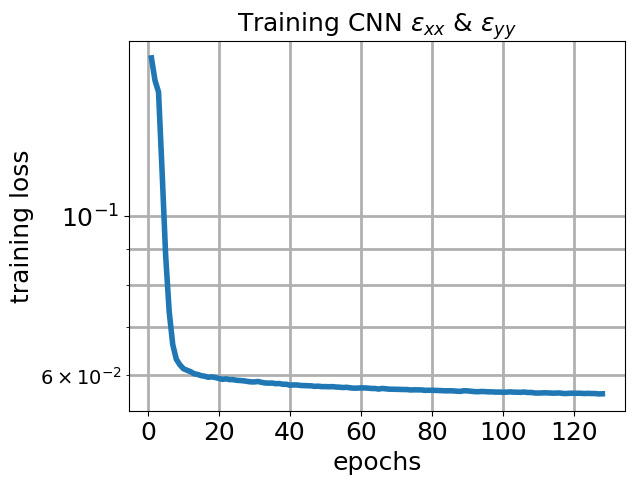
\includegraphics[totalheight=\nhgfigheight]{Figures/final1/training/exxeyy/field_strainxxyy_plot_loss.png}
    \caption{Training loss}
  \end{subfigure}
  %
  \begin{subfigure}[b]{0.45\linewidth}
    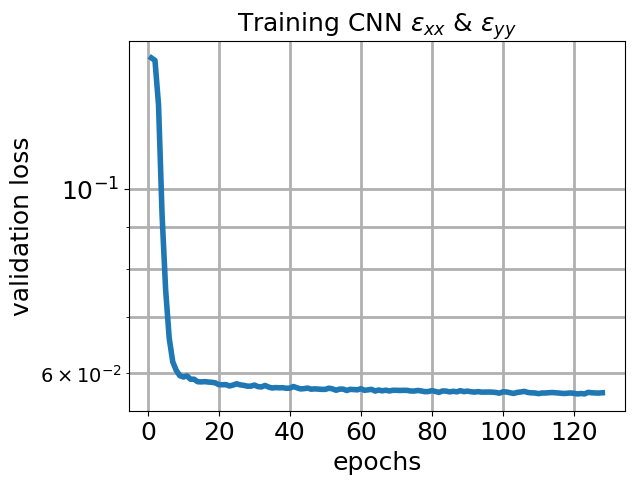
\includegraphics[totalheight=\nhgfigheight]{Figures/final1/training/exxeyy/field_strainxxyy_plot_val_loss.png}
    \caption{Validation loss}
  \end{subfigure}
  %
\caption{\label{fig:oneinc:trainexxeyy} Training curves for CNN $\epsilon_{xx}$ \& $\epsilon_{yy}$ for imaging one inclusion.}
\end{figure}
% oneinc: Training loss, val_loss for eyy
\begin{figure}[h]
  %
  \centering
  \begin{subfigure}[b]{0.45\linewidth}
    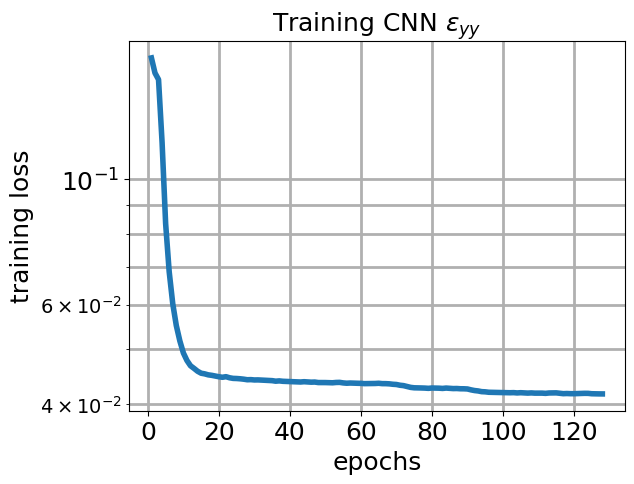
\includegraphics[totalheight=\nhgfigheight]{Figures/final1/training/eyy/field_strainyy_plot_loss.png}
    \caption{Training loss}
  \end{subfigure}
  %
  \begin{subfigure}[b]{0.45\linewidth}
    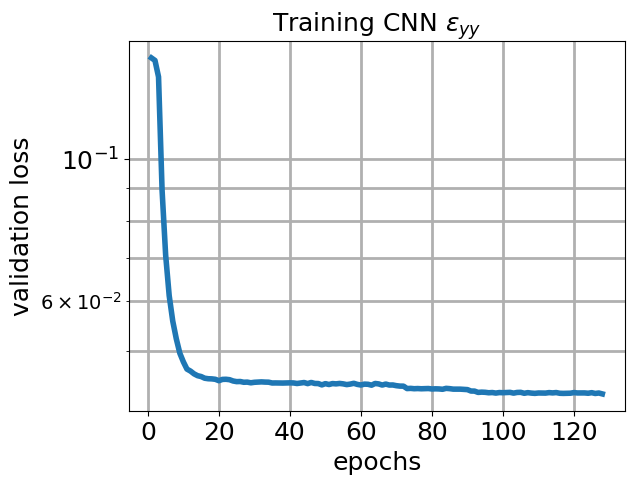
\includegraphics[totalheight=\nhgfigheight]{Figures/final1/training/eyy/field_strainyy_plot_val_loss.png}
    \caption{Validation loss}
  \end{subfigure}
  %
\caption{\label{fig:oneinc:traineyy} Training curves for CNN $\epsilon_{yy}$ for imaging one inclusion.}
\end{figure} 
% oneinc: Training loss, val_loss for uxuy
\begin{figure}[h]
  %
  \centering
  \begin{subfigure}[b]{0.45\linewidth}
    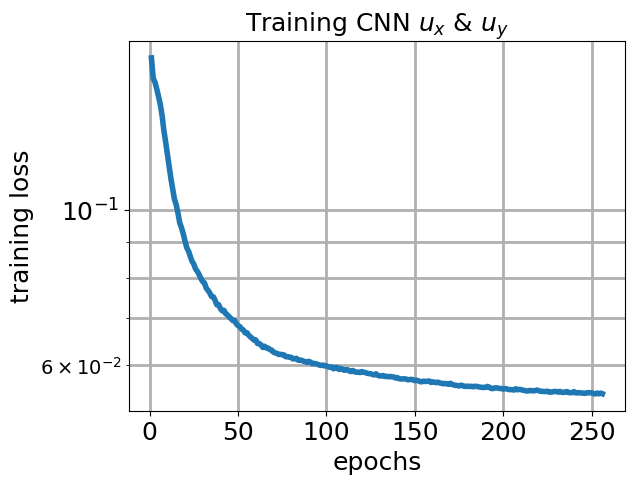
\includegraphics[totalheight=\nhgfigheight]{Figures/final1/training/uxuy/field_images_plot_loss.png}
    \caption{Training loss}
  \end{subfigure}
  %
  \begin{subfigure}[b]{0.45\linewidth}
    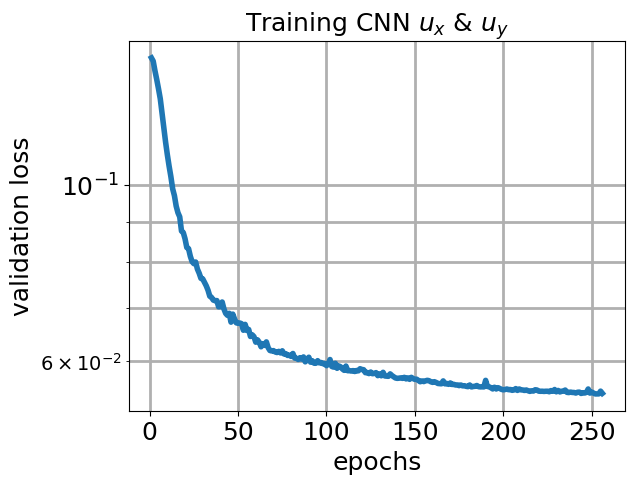
\includegraphics[totalheight=\nhgfigheight]{Figures/final1/training/uxuy/field_images_plot_val_loss.png}
    \caption{Validation loss}
  \end{subfigure}
  %
  \caption{\label{fig:oneinc:trainuxuy} Training curves for CNN $u_x$ \& $u_y$ for imaging one inclusion.}
\end{figure}
% oneinc: Training loss, val_loss for uy
\begin{figure}[h]
  %
  \centering
  \begin{subfigure}[b]{0.45\linewidth}
    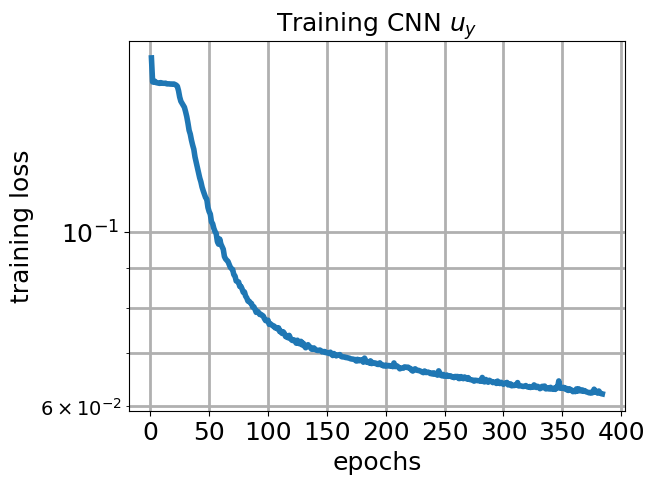
\includegraphics[totalheight=\nhgfigheight]{Figures/final1/training/uy/field_imagesy_plot_loss.png}
    \caption{Training loss}
  \end{subfigure}
  %
  \begin{subfigure}[b]{0.45\linewidth}
    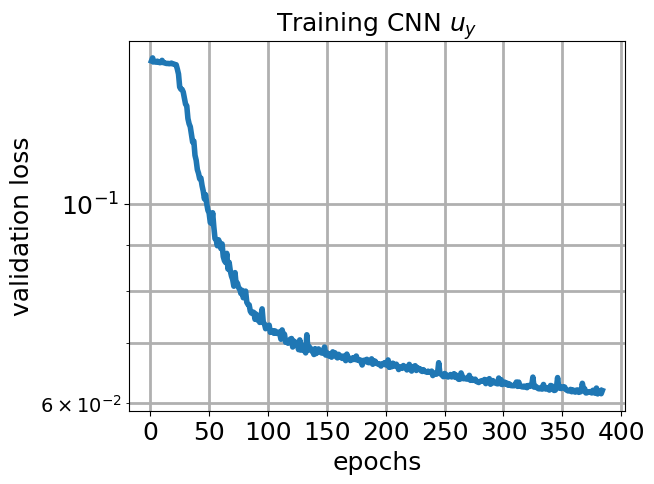
\includegraphics[totalheight=\nhgfigheight]{Figures/final1/training/uy/field_imagesy_plot_val_loss.png}
    \caption{Validation loss}
  \end{subfigure}
  %
  \caption{\label{fig:oneinc:trainuy} Training curves for CNN $u_y$ for imaging one inclusion.}
\end{figure}
%
% oneinctanh: Training loss, val_loss for exxeyy
\begin{figure}[h]
  %
  \centering
  \begin{subfigure}[b]{0.45\linewidth}
    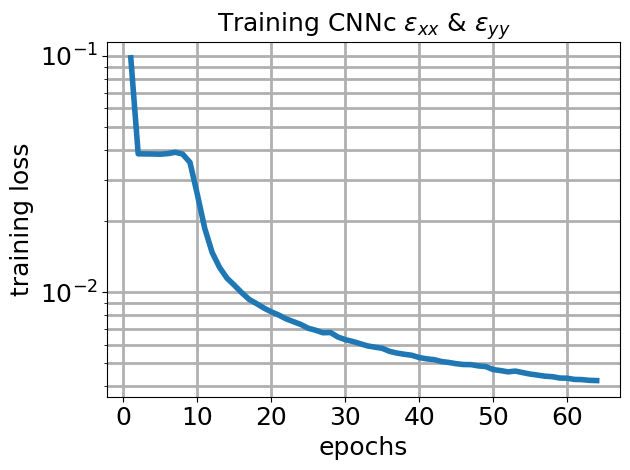
\includegraphics[totalheight=\nhgfigheight]{Figures/final1c/training/exxeyy/field_strainxxyy_plot_loss.png}
    \caption{Training loss}
  \end{subfigure}
  %
  \begin{subfigure}[b]{0.45\linewidth}
    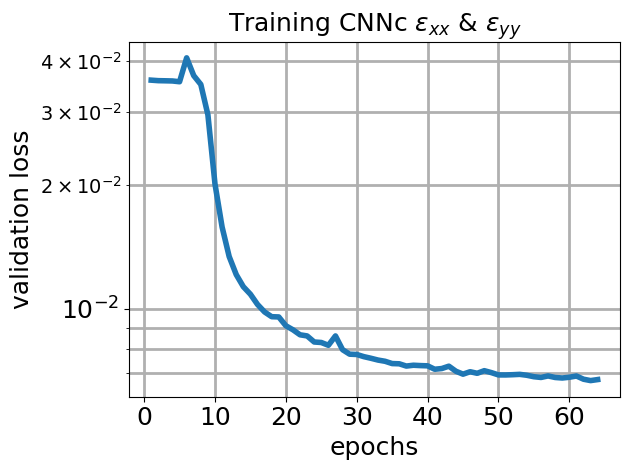
\includegraphics[totalheight=\nhgfigheight]{Figures/final1c/training/exxeyy/field_strainxxyy_plot_val_loss.png}
    \caption{Validation loss}
  \end{subfigure}
  %
\caption{\label{fig:oneinctanh:trainexxeyy} Training curves for CNNc $\epsilon_{xx}$ \& $\epsilon_{yy}$ for imaging one inclusion.}
\end{figure}
% oneinctanh: Training loss, val_loss for eyy
\begin{figure}[h]
  %
  \centering
  \begin{subfigure}[b]{0.45\linewidth}
    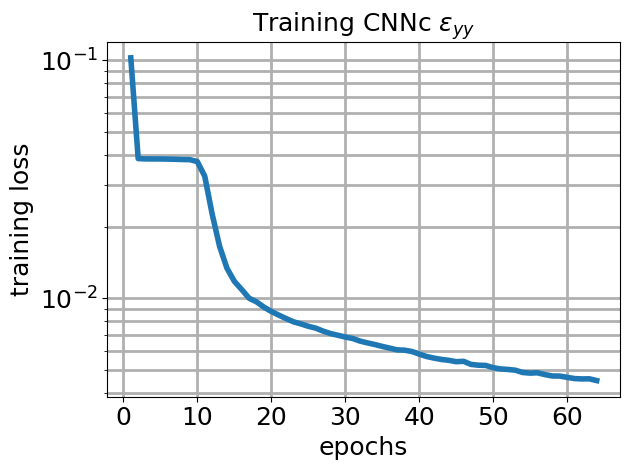
\includegraphics[totalheight=\nhgfigheight]{Figures/final1c/training/eyy/field_strainyy_plot_loss.png}
    \caption{Training loss}
  \end{subfigure}
  %
  \begin{subfigure}[b]{0.45\linewidth}
    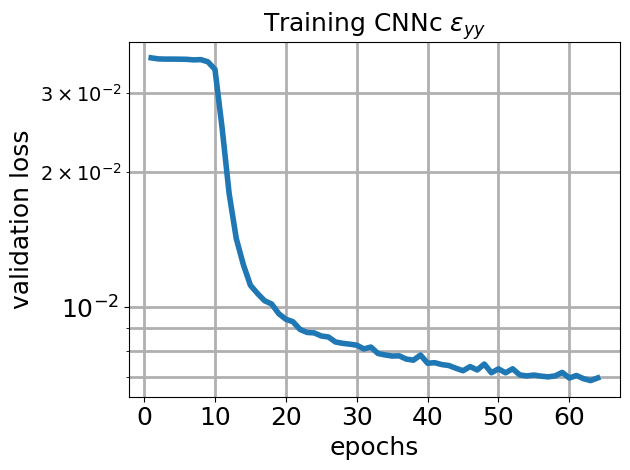
\includegraphics[totalheight=\nhgfigheight]{Figures/final1c/training/eyy/field_strainyy_plot_val_loss.png}
    \caption{Validation loss}
  \end{subfigure}
  %
\caption{\label{fig:oneinctanh:traineyy} Training curves for CNNc $\epsilon_{yy}$ for imaging one inclusion.}
\end{figure}
%
% oneinctanh: Training loss, val_loss for ux+uy
\begin{figure}[h]
  %
  \centering
  \begin{subfigure}[b]{0.45\linewidth}
    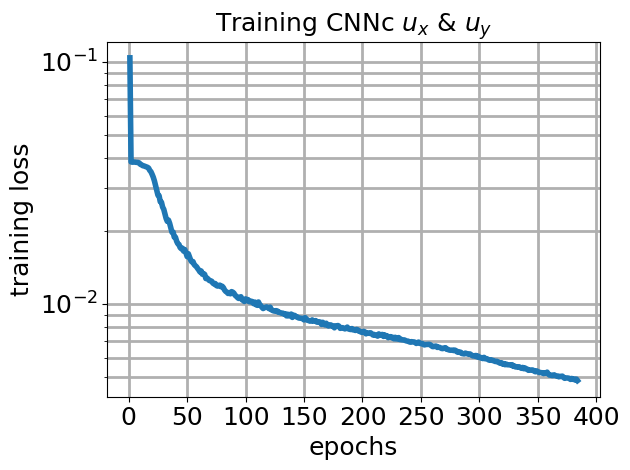
\includegraphics[totalheight=\nhgfigheight]{Figures/final1c/training/uxuy/field_images_plot_loss.png}
    \caption{Training loss}
  \end{subfigure}
  %
  \begin{subfigure}[b]{0.45\linewidth}
    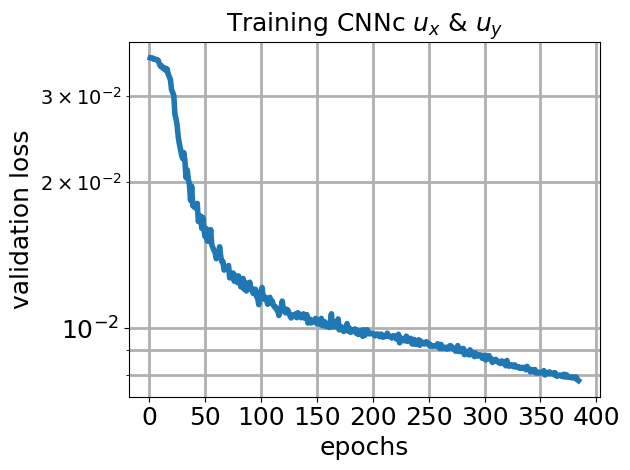
\includegraphics[totalheight=\nhgfigheight]{Figures/final1c/training/uxuy/field_images_plot_val_loss.png}
    \caption{Validation loss}
  \end{subfigure}
  %
\caption{\label{fig:oneinctanh:trainuxuy} Training curves for CNNc $u_x$ \& $u_y$ for imaging one inclusion.}
\end{figure}
%
% oneinctanh: Training loss, val_loss for uy
\begin{figure}[h]
  %
  \centering
  \begin{subfigure}[b]{0.45\linewidth}
    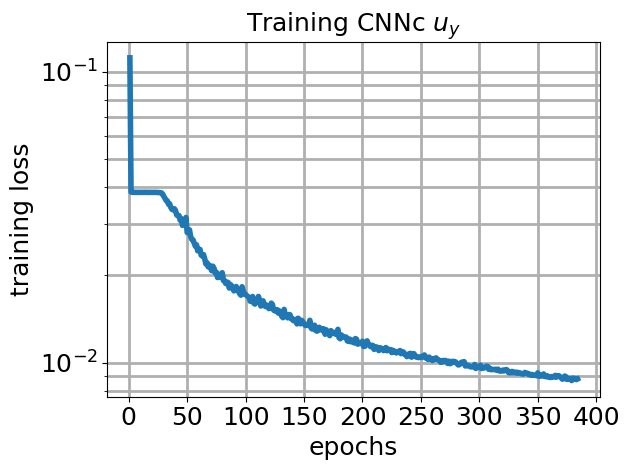
\includegraphics[totalheight=\nhgfigheight]{Figures/final1c/training/uy/field_imagesy_plot_loss.png}
    \caption{Training loss}
  \end{subfigure}
  %
  \begin{subfigure}[b]{0.45\linewidth}
    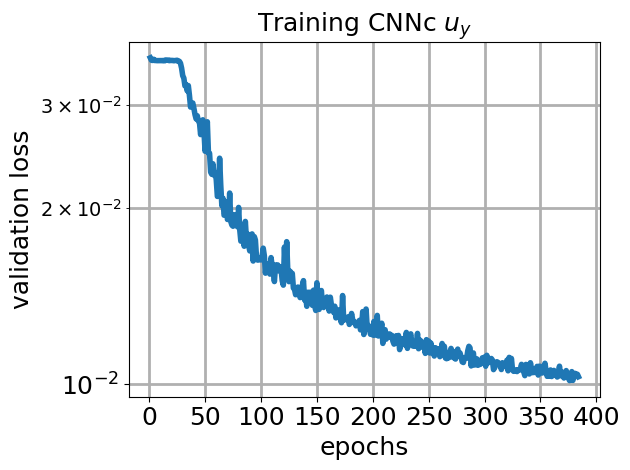
\includegraphics[totalheight=\nhgfigheight]{Figures/final1c/training/uy/field_imagesy_plot_val_loss.png}
    \caption{Validation loss}
  \end{subfigure}
  %
\caption{\label{fig:oneinctanh:trainuy} Training curves for CNNc $u_y$ for imaging one inclusion.}
\end{figure}
% Figure 1 (softplus)
\begin{figure}[h]
  \mupics{1}{1}{fig:oneinc:1}
  \caption{\label{fig:oneinc:1}Imaging one inclusion (softplus): result 1. These results show that the shear modulus of small inclusions is underpredicted. Result (d) is more accurate than result (a) in spite of using only $\epsilon_{yy}$. There are areas of low shear modulus adjacent to the inclusion especially in figures (b) and (c). See Table (\ref{tab:subcap}) for an explanation of the subcaptions.}
\end{figure}
\newpage
\clearpage
% Figure 1 (onetanh)
\begin{figure}[h]
  \mupics{1c}{1}{fig:oneinctanh:1}
  \caption{\label{fig:oneinctanh:1}Imaging one inclusion (twisted tanh): result 1. Results (a)-(d) are fairly accurate. Results (f)-(i) underpredict the shear modulus but are still better than the softplus results. See Table (\ref{tab:subcap}) for an explanation of the subcaptions.}
\end{figure}
\newpage
\clearpage
% Figure 2 (softplus)
\begin{figure}[h]
  \mupics{1}{2}{fig:oneinc:2}
  \caption{\label{fig:oneinc:2}Imaging one inclusion (softplus): result 2. These results show that the shear modulus of larger inclusions is overpredicted using strain data. There are areas of low shear modulus adjacent to the inclusion especially in figures (b) and (c). See Table (\ref{tab:subcap}) for an explanation of the subcaptions.}
\end{figure}
\newpage
\clearpage
% Figure 2 (onetanh)
\begin{figure}[h]
  \mupics{1c}{2}{fig:oneinctanh:2}
  \caption{\label{fig:oneinctanh:2}Imaging one inclusion (twisted tanh): result 2. These results are more accurate than the results using the softplus activation. The results do not show areas of low shear modulus adjacent to the inclusions. See Table (\ref{tab:subcap}) for an explanation of the subcaptions.}
\end{figure}
\newpage
\clearpage
% Figure 3 (softplus)
\begin{figure}[h]
  \mupics{1}{3}{fig:oneinc:3}
  \caption{\label{fig:oneinc:3}Imaging one inclusion (softplus): result 3. Again, these results show that the shear modulus of small inclusions is underpredicted. There are areas of low shear modulus adjacent to the inclusion especially in figures (b) and (c). See Table (\ref{tab:subcap}) for an explanation of the subcaptions.}
\end{figure}
\newpage
\clearpage
% Figure 3 (onetanh)
\begin{figure}[h]
  \mupics{1c}{3}{fig:oneinctanh:3}
  \caption{\label{fig:oneinctanh:3}Imaging one inclusion (twisted tanh): result 3. Results (b)-(g) are fairly accurate overall and certainly more accurate than the results using the softplus activation. There are no regions of low shear modulus adjacent to the inclusions. The shear modulus is under predicted in (h) and (i). See Table (\ref{tab:subcap}) for an explanation of the subcaptions.}
\end{figure}
\newpage
\clearpage
% Figure 4 (softplus)
\begin{figure}[h]
  \mupics{1}{4}{fig:oneinc:4}
  \caption{\label{fig:oneinc:4}Imaging one inclusion (softplus): result 4. Shear modulus of larger inclusions is over predicted. There are areas of low shear modulus adjacent to the inclusion especially in figures (b) and (c). See Table (\ref{tab:subcap}) for an explanation of the subcaptions.}
\end{figure}
\newpage
\clearpage
% Figure 4 (onetanh)
\begin{figure}[h]
  \mupics{1c}{4}{fig:oneinctanh:4}
  \caption{\label{fig:oneinctanh:4}Imaging one inclusion (twisted tanh): result 4. Results (b)-(e) are accurate. Results (f)-(i) show over prediction of the shear modulus. There are no regions of low shear modulus adjacent to the inclusions. See Table (\ref{tab:subcap}) for an explanation of the subcaptions.}
\end{figure}
\newpage
\clearpage
% Figure 5 (softplus)
\begin{figure}[h]
  \mupics{1}{5}{fig:oneinc:5}
  \caption{\label{fig:oneinc:5}Imaging one inclusion (softplus): result 5. Shear modulus of medium sized inclusion seems to be predicted reasonably accurately. There are areas of low shear modulus adjacent to the inclusion especially in figures (b) and (c). See Table (\ref{tab:subcap}) for an explanation of the subcaptions.}
\end{figure}
\newpage
\clearpage
% Figure 5 (onetanh)
\begin{figure}[h]
  \mupics{1c}{5}{fig:oneinctanh:5}
  \caption{\label{fig:oneinctanh:5}Imaging one inclusion (twisted tanh): result 5. The shear modulus is slightly over predicted in all figures. The best reconstruction is (i). There are no regions of low shear modulus adjacent to the inclusions. See Table (\ref{tab:subcap}) for an explanation of the subcaptions.} 
\end{figure}
\newpage
\clearpage
% Figure 6 (softplus)
\begin{figure}[h]
  \mupics{1}{6}{fig:oneinc:6}
  \caption{\label{fig:oneinc:6}Imaging one inclusion (softplus): result 6. Shear modulus of small inclusions is severely underpredicted. Apart from figures (d)-(e) there seems to be no sign of an inclusion in other figures. See Table (\ref{tab:subcap}) for an explanation of the subcaptions.}
\end{figure}
\newpage
\clearpage
% Figure 6 (onetanh)
\begin{figure}[h]
  \mupics{1c}{6}{fig:oneinctanh:6}
  \caption{\label{fig:oneinctanh:6}Imaging one inclusion (twisted tanh): result 6. The inclusion is present in figures (b)-(e) but its shear modulus is underpredicted. The inclusion is almost absent from figures (f)-(i). See Table (\ref{tab:subcap}) for an explanation of the subcaptions.}
\end{figure}
\newpage
\clearpage
% Figure 7 (softplus)
\begin{figure}[h]
  \mupics{1}{7}{fig:oneinc:7}
  \caption{\label{fig:oneinc:7}Imaging one inclusion (softplus): result 7. Shear modulus of this inclusion is slightly overpredicted. There are areas of low shear modulus adjacent to the inclusion especially in figures (b),(c) and (f)-(i). See Table (\ref{tab:subcap}) for an explanation of the subcaptions.}
\end{figure}
\newpage
\clearpage
% Figure 7 (onetanh)
\begin{figure}[h]
  \mupics{1c}{7}{fig:oneinctanh:7}
  \caption{\label{fig:oneinctanh:7}Imaging one inclusion (twisted tanh): result 7. The predictions are accurate in all cases. There are no regions of low shear modulus adjacent to the inclusions. See Table (\ref{tab:subcap}) for an explanation of the subcaptions.}
\end{figure}
\newpage
\clearpage
% Figure 8 (softplus)
\begin{figure}[h]
  \mupics{1}{8}{fig:oneinc:8}
  \caption{\label{fig:oneinc:8}Imaging one inclusion (softplus): result 8. Shear modulus of this small inclusion is severely underpredicted in all figures. There are regions of low shear modulus adjacent to the inclusion in figures (b),(c),(h) and (i). See Table (\ref{tab:subcap}) for an explanation of the subcaptions.}
\end{figure}
\newpage
\clearpage
% Figure 8 (onetanh)
\begin{figure}[h]
  \mupics{1c}{8}{fig:oneinctanh:8}
  \caption{\label{fig:oneinctanh:8}Imaging one inclusion (twisted tanh): result 8. Unlike the previous result with softplus, the inclusion is clearly visible in all figures. Result (b) is good and the results get progressively worse towards result (i). See Table (\ref{tab:subcap}) for an explanation of the subcaptions.}
\end{figure}
\newpage
\clearpage
% Figure 9 (softplus)
\begin{figure}[h]
  \mupics{1}{9}{fig:oneinc:9}
  \caption{\label{fig:oneinc:9}Imaging one inclusion (softplus): result 9. The shear modulus is underpredicted in all cases except (d) and (e). There are patches of low shear modulus around the predicted inclusions in all reconstructions. See Table (\ref{tab:subcap}) for an explanation of the subcaptions.}
\end{figure}
\newpage
\clearpage
% Figure 9 (onetanh)
\begin{figure}[h]
  \mupics{1c}{9}{fig:oneinctanh:9}
  \caption{\label{fig:oneinctanh:9}Imaging one inclusion (twisted tanh): result 9. The results are fairly accurate in all cases except (f) and (g) where the shear modulus is over predicted. See Table (\ref{tab:subcap}) for an explanation of the subcaptions.}
\end{figure}
\newpage
\clearpage
% Figure 10 (softplus)
\begin{figure}[h]
  \mupics{1}{10}{fig:oneinc:10}
  \caption{\label{fig:oneinc:10}Imaging one inclusion (softplus): result 10. Shear modulus of this small inclusion is under predicted. Surprisingly it is result (d) in which only $\epsilon_{yy}$ is used which is the best. See Table (\ref{tab:subcap}) for an explanation of the subcaptions.}
\end{figure}
\newpage
\clearpage
% Figure 10 (onetanh)
\begin{figure}[h]
  \mupics{1c}{10}{fig:oneinctanh:10}
  \caption{\label{fig:oneinctanh:10}Imaging one inclusion (twisted tanh): result 10. The results are more accurate than the softplus case. There is overprediction in (d)-(g), and underprediction in (h) and (i). See Table (\ref{tab:subcap}) for an explanation of the subcaptions.}
\end{figure}
\newpage
\clearpage
% Figure 11 (softplus)
\begin{figure}[h]
  \mupics{1}{11}{fig:oneinc:11}
  \caption{\label{fig:oneinc:11}Imaging one inclusion (softplus): result 11. Inclusions to the side of the domain seem to be detected fairly well. There is overprediction in (b)-(e). All the results, especially (b) and (c), show regions of low shear modulus adjacent to regions of high shear modulus. See Table (\ref{tab:subcap}) for an explanation of the subcaptions.}
\end{figure}
\newpage
\clearpage
% Figure 11 (onetanh)
\begin{figure}[h]
  \mupics{1c}{11}{fig:oneinctanh:11}
  \caption{\label{fig:oneinctanh:11}Imaging one inclusion (twisted tanh): result 11. All results are fairly accurate. There are ripples in the background in (f)-(g). See Table (\ref{tab:subcap}) for an explanation of the subcaptions.}
\end{figure}
\newpage
\clearpage
% Figure 12 (softplus)
\begin{figure}[h]
  \mupics{1}{12}{fig:oneinc:12}
  \caption{\label{fig:oneinc:12}Imaging one inclusion (softplus): result 12. This inclusion is detected fairly accurately. The shear modulus is slightly over-predicted. Figures (b) and (c), show regions of low shear modulus adjacent to regions of high shear modulus. See Table (\ref{tab:subcap}) for an explanation of the subcaptions.}
\end{figure}
\newpage
\clearpage
% Figure 12 (onetanh)
\begin{figure}[h]
  \mupics{1c}{12}{fig:oneinctanh:12}
  \caption{\label{fig:oneinctanh:12}Imaging one inclusion (twisted tanh): result 12. Results (b)-(e) are fairly accurate. There is over-prediction in (f)-(i). There are no regions of low shear modulus adjacent to regions of high shear modulus. See Table (\ref{tab:subcap}) for an explanation of the subcaptions.}
\end{figure}
\newpage
\clearpage
% Figure 13 (softplus)
\begin{figure}[h]
  \mupics{1}{13}{fig:oneinc:13}
  \caption{\label{fig:oneinc:13}Imaging one inclusion (softplus): result 13. There are pronounced regions of low shear modulus next to regions in figures (b) and (c). Surprisingly the best reconstruction is obtained in (d) where only $\epsilon_{yy}$ is used. See Table (\ref{tab:subcap}) for an explanation of the subcaptions.}
\end{figure}
\newpage
\clearpage
% Figure 13 (onetanh)
\begin{figure}[h]
  \mupics{1c}{13}{fig:oneinctanh:13}
  \caption{\label{fig:oneinctanh:13}Imaging one inclusion (twisted tanh): result 13. Results (b)-(g) are fairly accurate. However, there is overprediction in figures (h) and (i). See Table (\ref{tab:subcap}) for an explanation of the subcaptions.}
\end{figure}
\newpage
\clearpage
% Figure 14 (softplus)
\begin{figure}[h]
  \mupics{1}{14}{fig:oneinc:14}
  \caption{\label{fig:oneinc:14}Imaging one inclusion (softplus): result 14. Medium sized inclusions are detected fairly well. Surprisingly the best reconstruction is obtained in (d) where only $\epsilon_{yy}$ is used. See Table (\ref{tab:subcap}) for an explanation of the subcaptions.}
\end{figure}
\newpage
\clearpage
% Figure 14 (onetanh)
\begin{figure}[h]
  \mupics{1c}{14}{fig:oneinctanh:14}
  \caption{\label{fig:oneinctanh:14}Imaging one inclusion (twisted tanh): result 14. The inclusions are not clearly defined. They are fuzzy. This may be because the true shear modulus is low. See Table (\ref{tab:subcap}) for an explanation of the subcaptions.}
\end{figure}
\newpage
\clearpage
% Figure 15 (softplus)
\begin{figure}[h]
  \mupics{1}{15}{fig:oneinc:15}
  \caption{\label{fig:oneinc:15}Imaging one inclusion (softplus): result 15. Medium sized inclusions are detected fairly well. There is slight overprediction of the shear modulus. There are regions of low shear modulus adjacent to the inclusions. See Table (\ref{tab:subcap}) for an explanation of the subcaptions.}
\end{figure}
\newpage
\clearpage
% Figure 15 (onetanh)
\begin{figure}[h]
  \mupics{1c}{15}{fig:oneinctanh:15}
  \caption{\label{fig:oneinctanh:15}Imaging one inclusion (twisted tanh): result 15. Inclusions are detected clearly but their shear modulus is overpredicted. There are no regions of low shear modulus adjacent to the inclusion. See Table (\ref{tab:subcap}) for an explanation of the subcaptions.}
\end{figure}
\newpage
\clearpage
% Figure 16 (softplus)
\begin{figure}[h]
  \mupics{1}{16}{fig:oneinc:16}
  \caption{\label{fig:oneinc:16}Imaging one inclusion (softplus): result 16. Medium sized inclusions are detected fairly well.  There are pronounced regions of low shear modulus next to regions in figures (b) and (c). Surprisingly the best reconstruction is obtained in (d) where only $\epsilon_{yy}$ is used. See Table (\ref{tab:subcap}) for an explanation of the subcaptions.}
\end{figure}
\newpage
\clearpage
% Figure 16 (onetanh)
\begin{figure}[h]
  \mupics{1c}{16}{fig:oneinctanh:16}
  \caption{\label{fig:oneinctanh:16}Imaging one inclusion (twisted tanh): result 16. The inclusion is detected accurately in all figures. There are no regions of low shear modulus adjacent to the inclusions. See Table (\ref{tab:subcap}) for an explanation of the subcaptions.}
\end{figure}
\newpage
\clearpage
%
\section{\label{sect:threeinc}Imaging up to three inclusions}
In this section, we evaluate the ability of the CNN to learn from fields containing multiple (up to $3$) inclusions. The CNN architecture is exactly as described in Section (\ref{sect:cnnarch}). The problem setup is the same as described in Section (\ref{sect:probsetup}) with the following differences. There can be either $1$, $2$ or $3$ inclusions in the domain and their radius ranges from $0.1$ units to $0.15$ units. Training curves are presented in Figures (\ref{fig:threeinc:trainexxeyy}-\ref{fig:threeinctanh:trainuy}). Figures (\ref{fig:threeinc:1}-\ref{fig:threeinctanh:16}) show the results obtained. 
%
% Training loss, val_loss for exxeyy (3 softplus)
\begin{figure}[h]
  %
  \centering
  \begin{subfigure}[b]{0.45\linewidth}
    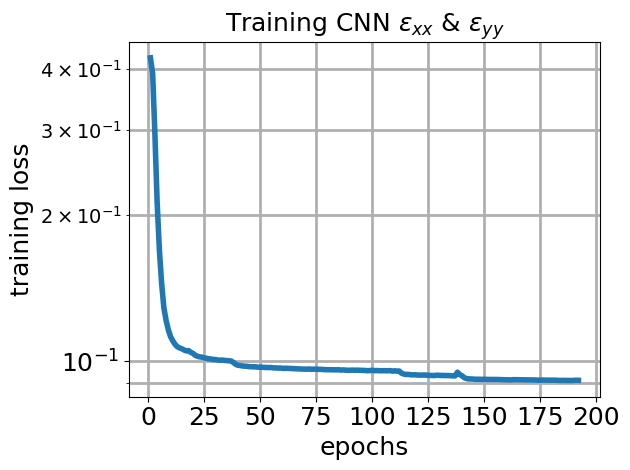
\includegraphics[totalheight=\nhgfigheight]{Figures/final3/training/exxeyy/field_strainxxyy_plot_loss.png}
    \caption{Training loss}
  \end{subfigure}
  %
  \begin{subfigure}[b]{0.45\linewidth}
    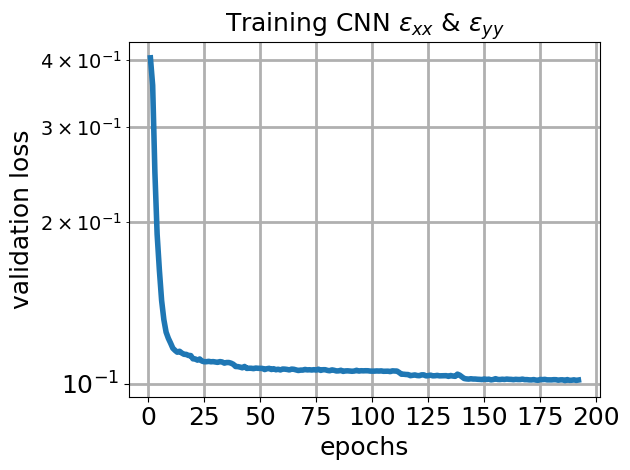
\includegraphics[totalheight=\nhgfigheight]{Figures/final3/training/exxeyy/field_strainxxyy_plot_val_loss.png}
    \caption{Validation loss}
  \end{subfigure}
  %
\caption{\label{fig:threeinc:trainexxeyy} Training curves for CNN $\epsilon_{xx}$ \& $\epsilon_{yy}$ for imaging up to 3 inclusions.}
\end{figure}
% Training loss, val_loss for eyy (3 softplus)
\begin{figure}[h]
  %
  \centering
  \begin{subfigure}[b]{0.45\linewidth}
    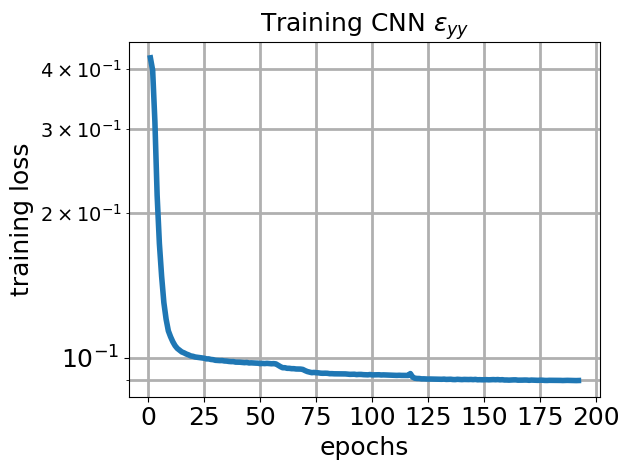
\includegraphics[totalheight=\nhgfigheight]{Figures/final3/training/eyy/field_strainyy_plot_loss.png}
    \caption{Training loss}
  \end{subfigure}
  %
  \begin{subfigure}[b]{0.45\linewidth}
    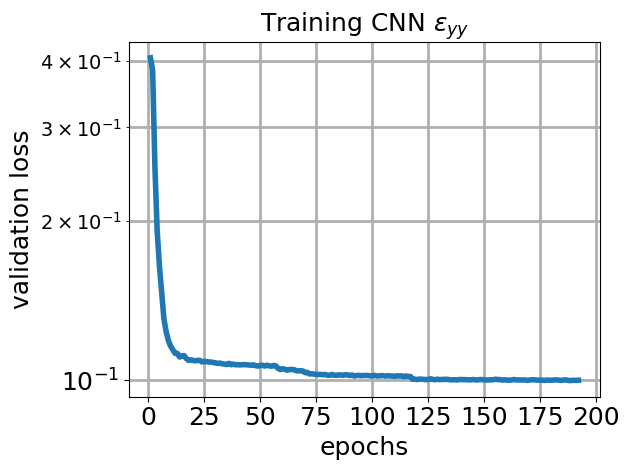
\includegraphics[totalheight=\nhgfigheight]{Figures/final3/training/eyy/field_strainyy_plot_val_loss.png}
    \caption{Validation loss}
  \end{subfigure}
  %
\caption{\label{fig:threeinc:traineyy} Training curves for CNN $\epsilon_{yy}$ for imaging up to 3 inclusions.}
\end{figure} 
% Training loss, val_loss for uxuy (3 softplus)
\begin{figure}[h]
  %
  \centering
  \begin{subfigure}[b]{0.45\linewidth}
    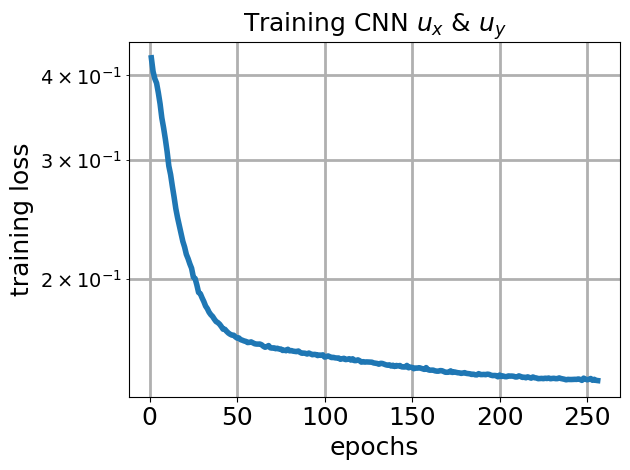
\includegraphics[totalheight=\nhgfigheight]{Figures/final3/training/uxuy/field_images_plot_loss.png}
    \caption{Training loss}
  \end{subfigure}
  %
  \begin{subfigure}[b]{0.45\linewidth}
    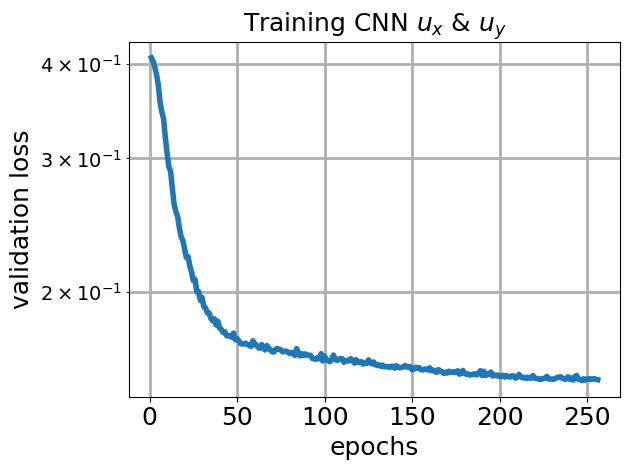
\includegraphics[totalheight=\nhgfigheight]{Figures/final3/training/uxuy/field_images_plot_val_loss.png}
    \caption{Validation loss}
  \end{subfigure}
  %
  \caption{\label{fig:threeinc:trainuxuy} Training curves for CNN $u_x$ \& $u_y$ for imaging up to 3 inclusions.}
\end{figure}
% Training loss, val_loss for uy (3 softplus)
\begin{figure}[h]
  %
  \centering
  \begin{subfigure}[b]{0.45\linewidth}
    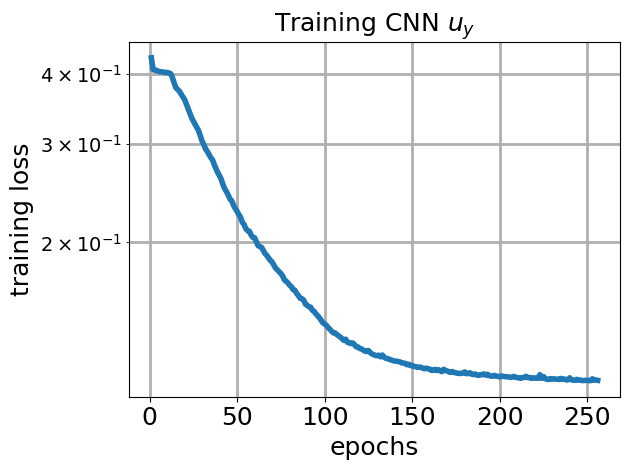
\includegraphics[totalheight=\nhgfigheight]{Figures/final3/training/uy/field_imagesy_plot_loss.png}
    \caption{Training loss}
  \end{subfigure}
  %
  \begin{subfigure}[b]{0.45\linewidth}
    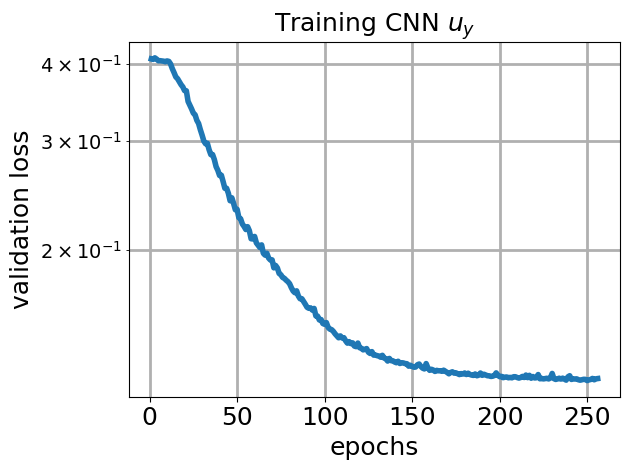
\includegraphics[totalheight=\nhgfigheight]{Figures/final3/training/uy/field_imagesy_plot_val_loss.png}
    \caption{Validation loss}
  \end{subfigure}
  %
  \caption{\label{fig:threeinc:trainuy} Training curves for CNN $u_y$ for imaging up to 3 inclusions.}
\end{figure}
%
% Training loss, val_loss for exxeyy (3 tanh)
\begin{figure}[h]
  %
  \centering
  \begin{subfigure}[b]{0.45\linewidth}
    \includegraphics[totalheight=\nhgfigheight]{Figures/final3c/training/exxeyy/field_strainxxyy_plot_loss.png}
    \caption{Training loss}
  \end{subfigure}
  %
  \begin{subfigure}[b]{0.45\linewidth}
    \includegraphics[totalheight=\nhgfigheight]{Figures/final3c/training/exxeyy/field_strainxxyy_plot_val_loss.png}
    \caption{Validation loss}
  \end{subfigure}
  %
\caption{\label{fig:threeinctanh:trainexxeyy} Training curves for CNNc $\epsilon_{xx}$ \& $\epsilon_{yy}$ for imaging three inclusions with constraints.}
\end{figure}
% Training loss, val_loss for eyy (3 tanh)
\begin{figure}[h]
  %
  \centering
  \begin{subfigure}[b]{0.45\linewidth}
    \includegraphics[totalheight=\nhgfigheight]{Figures/final3c/training/eyy/field_strainyy_plot_loss.png}
    \caption{Training loss}
  \end{subfigure}
  %
  \begin{subfigure}[b]{0.45\linewidth}
    \includegraphics[totalheight=\nhgfigheight]{Figures/final3c/training/eyy/field_strainyy_plot_val_loss.png}
    \caption{Validation loss}
  \end{subfigure}
  %
\caption{\label{fig:threeinctanh:traineyy} Training curves for CNNc $\epsilon_{yy}$ for imaging three inclusions with constraints.}
\end{figure}
%
% Training loss, val_loss for ux+uy (3 tanh)
\begin{figure}[h]
  %
  \centering
  \begin{subfigure}[b]{0.45\linewidth}
    \includegraphics[totalheight=\nhgfigheight]{Figures/final3c/training/uxuy/field_images_plot_loss.png}
    \caption{Training loss}
  \end{subfigure}
  %
  \begin{subfigure}[b]{0.45\linewidth}
    \includegraphics[totalheight=\nhgfigheight]{Figures/final3c/training/uxuy/field_images_plot_val_loss.png}
    \caption{Validation loss}
  \end{subfigure}
  %
  \caption{\label{fig:threeinctanh:trainuxuy} Training curves for CNNc $u_x$ \& $u_y$ for imaging three inclusions with constraints.}
\end{figure}
% Training loss, val_loss for uy (3 tanh)
\begin{figure}[h]
  %
  \centering
  \begin{subfigure}[b]{0.45\linewidth}
    \includegraphics[totalheight=\nhgfigheight]{Figures/final3c/training/uy/field_imagesy_plot_loss.png}
    \caption{Training loss}
  \end{subfigure}
  %
  \begin{subfigure}[b]{0.45\linewidth}
    \includegraphics[totalheight=\nhgfigheight]{Figures/final3c/training/uy/field_imagesy_plot_val_loss.png}
    \caption{Validation loss}
  \end{subfigure}
  %
\caption{\label{fig:threeinctanh:trainuy} Training curves for CNNc $u_y$ for imaging three inclusions with constraints.}
\end{figure}
% Reconstructions
% Figure 1 3inc
\begin{figure}[h]
  \mupics{3}{1}{fig:threeinc:1}
  \caption{\label{fig:threeinc:1}Imaging up to 3 inclusions (softplus): result 1. The inclusion with the higher shear modulus is clearly captured. The inclusion with the lower shear modulus is not captured clearly. There are regions of low shear modulus adjacent to the inclusion. See Table (\ref{tab:subcap}) for an explanation of the subcaptions.}
\end{figure}
\newpage
\clearpage
% Figure 1 (threetanh)
\begin{figure}[h]
  \mupics{3c}{1}{fig:threeinctanh:1}
  \caption{\label{fig:threeinctanh:1}Imaging up to 3 inclusions (twisted tanh): result 1. The inclusion with the higher shear modulus is overpredicted. The inclusion with the lower shear modulus is not captured. There are no regions of low shear modulus adjacent to the inclusion. See Table (\ref{tab:subcap}) for an explanation of the subcaptions.}
\end{figure}
\newpage
\clearpage
% Figure 2 3inc
\begin{figure}[h]
  \mupics{3}{2}{fig:threeinc:2}
  \caption{\label{fig:threeinc:2}Imaging up to 3 inclusions (softplus) : result 2. The inclusion is clear but the shear modulus is overpredicted. There are regions of low shear modulus adjacent to the inclusion. See Table (\ref{tab:subcap}) for an explanation of the subcaptions.}
\end{figure}
\newpage
\clearpage
% Figure 2 (threetanh)
\begin{figure}[h]
  \mupics{3c}{2}{fig:threeinctanh:2}
  \caption{\label{fig:threeinctanh:2}Imaging up to 3 inclusions (twisted tanh) : result 2. The inclusion is clear but its shear modulus is slightly overpredicted. There are no regions of low shear modulus adjacent to the inclusion. See Table (\ref{tab:subcap}) for an explanation of the subcaptions.}
\end{figure}
\newpage
\clearpage
% Figure 3 3inc
\begin{figure}[h]
  \mupics{3}{3}{fig:threeinc:3}
  \caption{\label{fig:threeinc:3}Imaging up to 3 inclusions (softplus): result 3. The inclusions with the highest and second highest shear modulus are clearly visible and are slightly overpredicted. The inclusion with the lowest shear modulus is not clearly seen. There are regions of low shear modulus adjacent to the inclusion. See Table (\ref{tab:subcap}) for an explanation of the subcaptions.}
\end{figure}
\newpage
\clearpage
% Figure 3 (threetanh)
\begin{figure}[h]
  \mupics{3c}{3}{fig:threeinctanh:3}
  \caption{\label{fig:threeinctanh:3}Imaging up to 3 inclusions (twisted tanh) : result 3. The inclusions with the highest and second highest shear modulus are clearly visible and are slightly overpredicted in figures (b)-(g). Figures (h) and (i) show only the central inclusion clearly. The inclusion with the lowest shear modulus is not seen. See Table (\ref{tab:subcap}) for an explanation of the subcaptions.}
\end{figure}
\newpage
\clearpage
% Figure 4 3inc
\begin{figure}[h]
  \mupics{3}{4}{fig:threeinc:4}
  \caption{\label{fig:threeinc:4}Imaging up to 3 inclusions (softplus): result 4. The inclusion is clear but the shear modulus is overpredicted. There are regions of low shear modulus adjacent to the inclusion. See Table (\ref{tab:subcap}) for an explanation of the subcaptions.}
\end{figure}
\newpage
\clearpage
% Figure 4 (threetanh)
\begin{figure}[h]
  \mupics{3c}{4}{fig:threeinctanh:4}
  \caption{\label{fig:threeinctanh:4}Imaging up to 3 inclusions (twisted tanh): result 4. The inclusion is clear and the shear modulus is accurately predicted in (b)-(e). It is overpredicted in (f)-(i). There are no regions of low shear modulus adjacent to the inclusion. See Table (\ref{tab:subcap}) for an explanation of the subcaptions.}
\end{figure}
\newpage
\clearpage
% Figure 5 3inc
\begin{figure}[h]
  \mupics{3}{5}{fig:threeinc:5}
  \caption{\label{fig:threeinc:5}Imaging up to 3 inclusions (softplus): result 5. The overlapping inclusions are combined into a single inclusion whose shear modulus is overpredicted. The shear modulus of the inclusion to the right is accurately predicted. There are regions of low shear modulus adjacent to the inclusion. See Table (\ref{tab:subcap}) for an explanation of the subcaptions.}
\end{figure}
\newpage
\clearpage
% Figure 5 (threetanh)
\begin{figure}[h]
  \mupics{3c}{5}{fig:threeinctanh:5}
  \caption{\label{fig:threeinctanh:5}Imaging up to 3 inclusions (twisted tanh): result 5. The overlapping inclusions are combined into a single inclusion whose shear modulus is accurately predicted. The shear modulus of the inclusion to the right is accurately predicted. There are no regions of low shear modulus adjacent to the inclusion. See Table (\ref{tab:subcap}) for an explanation of the subcaptions.}
\end{figure}
\newpage
\clearpage
% Figure 6 3inc
\begin{figure}[h]
  \mupics{3}{6}{fig:threeinc:6}
  \caption{\label{fig:threeinc:6}Imaging up to 3 inclusions (softplus): result 6. The shear modulus of the top inclusion is accurately predicted while that of the lower inclusions is over predicted. There are regions of low shear modulus adjacent to the inclusion. See Table (\ref{tab:subcap}) for an explanation of the subcaptions.}
\end{figure}
\newpage
\clearpage
% Figure 6 (threetanh)
\begin{figure}[h]
  \mupics{3c}{6}{fig:threeinctanh:6}
  \caption{\label{fig:threeinctanh:6}Imaging up to 3 inclusions (twisted tanh): result 6. The shear modulus of the top inclusion is accurately predicted in (b)-(g) while that of the lower inclusions is over predicted. There are no regions of low shear modulus adjacent to the inclusion. The geometry of the top inclusion is not clearly predicted. It is seen only as wisps. See Table (\ref{tab:subcap}) for an explanation of the subcaptions.}
\end{figure}
\newpage
\clearpage
% Figure 7 3inc
\begin{figure}[h]
  \mupics{3}{7}{fig:threeinc:7}
  \caption{\label{fig:threeinc:7}Imaging up to 3 inclusions (softplus): result 7.  The overlapping inclusions are combined into a single inclusion whose shear modulus is overpredicted. There are regions of low shear modulus adjacent to the inclusion. See Table (\ref{tab:subcap}) for an explanation of the subcaptions.}
\end{figure}
\newpage
\clearpage
% Figure 7 (threetanh)
\begin{figure}[h]
  \mupics{3c}{7}{fig:threeinctanh:7}
  \caption{\label{fig:threeinctanh:7}Imaging up to 3 inclusions (twisted tanh): result 7. The overlapping inclusions are combined into a single inclusion whose shear modulus is slightly overpredicted. There are no regions of low shear modulus adjacent to the inclusion. See Table (\ref{tab:subcap}) for an explanation of the subcaptions.}
\end{figure}
\newpage
\clearpage
% Figure 8 3inc
\begin{figure}[h]
  \mupics{3}{8}{fig:threeinc:8}
  \caption{\label{fig:threeinc:8}Imaging up to 3 inclusions (softplus): result 8. The shear modulus of both inclusions is overpredicted. There are regions of low shear modulus adjacent to the inclusion, especially in (f),(h) and (i). See Table (\ref{tab:subcap}) for an explanation of the subcaptions.}
\end{figure}
\newpage
\clearpage
% Figure 8 (threetanh)
\begin{figure}[h]
  \mupics{3c}{8}{fig:threeinctanh:8}
  \caption{\label{fig:threeinctanh:8}Imaging up to 3 inclusions (twisted tanh): result 8. The shear modulus of both inclusions is overpredicted. There are no regions of low shear modulus adjacent to the inclusion. See Table (\ref{tab:subcap}) for an explanation of the subcaptions.}
\end{figure}
\newpage
\clearpage
% Figure 9 3inc
\begin{figure}[h]
  \mupics{3}{9}{fig:threeinc:9}
  \caption{\label{fig:threeinc:9}Imaging up to 3 inclusions (softplus): result 9. All three inclusions are clearly seen. The shear modulus of the top two is overpredicted while that of the lowest one is underpredicted. There are regions of low shear modulus adjacent to the inclusion. See Table (\ref{tab:subcap}) for an explanation of the subcaptions.}
\end{figure}
\newpage
\clearpage
% Figure 9 (threetanh)
\begin{figure}[h]
  \mupics{3c}{9}{fig:threeinctanh:9}
  \caption{\label{fig:threeinctanh:9}Imaging up to 3 inclusions (twisted tanh): result 9. The upper and central inclusions are clearly seen and their shear modulus is overpredicted. The lower inclusion is not clearly seen. It is seen only in wisps. There are no regions of low shear modulus adjacent to the inclusion. See Table (\ref{tab:subcap}) for an explanation of the subcaptions.}
\end{figure}
\newpage
\clearpage
% Figure 10 3inc
\begin{figure}[h]
  \mupics{3}{10}{fig:threeinc:10}
  \caption{\label{fig:threeinc:10}Imaging up to 3 inclusions (softplus): result 10. The inclusion is clearly seen but its shear modulus is overpredicted. There are regions of low shear modulus adjacent to the inclusion. See Table (\ref{tab:subcap}) for an explanation of the subcaptions.}
\end{figure}
\newpage
\clearpage
% Figure 10 (threetanh)
\begin{figure}[h]
  \mupics{3c}{10}{fig:threeinctanh:10}
  \caption{\label{fig:threeinctanh:10}Imaging up to 3 inclusions (twisted tanh): result 10. The inclusion is clearly seen but its shear modulus is overpredicted. There are no regions of low shear modulus adjacent to the inclusion. See Table (\ref{tab:subcap}) for an explanation of the subcaptions.}
\end{figure}
\newpage
\clearpage
% Figure 11 3inc
\begin{figure}[h]
  \mupics{3}{11}{fig:threeinc:11}
  \caption{\label{fig:threeinc:11}Imaging up to 3 inclusions (softplus): result 11. The inclusions are clearly seen. Their shear modulus is overpredicted. The predicted shear modulus of the inclusion with lower shear modulus is lower than the predicted shear modulus of the inclusion with higher shear modulus. That is, the relative contrast is predicted correctly. There are regions of low shear modulus adjacent to the inclusion. See Table (\ref{tab:subcap}) for an explanation of the subcaptions.}
\end{figure}
\newpage
\clearpage
% Figure 11 (threetanh)
\begin{figure}[h]
  \mupics{3c}{11}{fig:threeinctanh:11}
  \caption{\label{fig:threeinctanh:11}Imaging up to 3 inclusions (twisted tanh): result 11. Both inclusions are clearly seen but their shear modulii are overpredicted. There are no regions of low shear modulus adjacent to the inclusion. See Table (\ref{tab:subcap}) for an explanation of the subcaptions.}
\end{figure}
\newpage
\clearpage
% Figure 12 3inc
\begin{figure}[h]
  \mupics{3}{12}{}
  \caption{\label{fig:threeinc:12}Imaging up to 3 inclusions (softplus): result 12. The two overlapping inclusions are combined into one single inclusion whose shear modulus is slightly overpredicted. The predicted shear modulus of the top inclusion is approximately correct. There are regions of low shear modulus adjacent to the inclusions. See Table (\ref{tab:subcap}) for an explanation of the subcaptions.}
\end{figure}
\newpage
\clearpage
% Figure 12 (threetanh)
\begin{figure}[h]
  \mupics{3c}{12}{fig:threeinctanh:12}
  \caption{\label{fig:threeinctanh:12}Imaging up to 3 inclusions (twisted tanh): result 12. The two overlapping inclusions are combined into one single inclusion whose shear modulus is accurately predicted. The upper inclusion is not clearly seen. It is seen only in wisps. There are no regions of low shear modulus adjacent to the inclusion. See Table (\ref{tab:subcap}) for an explanation of the subcaptions.}
\end{figure}
\newpage
\clearpage
% Figure 13 3inc
\begin{figure}[h]
  \mupics{3}{13}{fig:threeinc:13}
  \caption{\label{fig:threeinc:13}Imaging up to 3 inclusions (softplus): result 13. The inclusion is clearly seen and its shear modulus is overpredicted. There are regions of low shear modulus adjacent to the inclusion. See Table (\ref{tab:subcap}) for an explanation of the subcaptions.}
\end{figure}
\newpage
\clearpage
% Figure 13 (threetanh)
\begin{figure}[h]
  \mupics{3c}{13}{fig:threeinctanh:13}
  \caption{\label{fig:threeinctanh:13}Imaging up to 3 inclusions (twisted tanh): result 13. The inclusion is clearly seen and its shear modulus is overpredicted. There are no regions of low shear modulus adjacent to the inclusion. See Table (\ref{tab:subcap}) for an explanation of the subcaptions.}
\end{figure}
\newpage
\clearpage
% Figure 14 3inc
\begin{figure}[h]
  \mupics{3}{14}{fig:threeinc:14}
  \caption{\label{fig:threeinc:14}Imaging up to 3 inclusions (softplus): result 14. The two inclusions are clearly seen. Their shear modulus is slightly overpredicted. The predicted shear modulus of the inclusion with lower shear modulus is lower than the predicted shear modulus of the inclusion with higher shear modulus. That is, the relative contrast is predicted correctly. There are regions of low shear modulus adjacent to the inclusion. See Table (\ref{tab:subcap}) for an explanation of the subcaptions.}
\end{figure}
\newpage
\clearpage
% Figure 14 (threetanh)
\begin{figure}[h]
  \mupics{3c}{14}{fig:threeinctanh:14}
  \caption{\label{fig:threeinctanh:14}Imaging up to 3 inclusions (twisted tanh): result 14. The two inclusions are clearly seen. Their shear modulus is slightly overpredicted. The predicted shear modulus of the inclusion with lower shear modulus is about the same as the predicted shear modulus of the inclusion with higher shear modulus. That is, the relative contrast is not predicted correctly. There are no regions of low shear modulus adjacent to the inclusion. See Table (\ref{tab:subcap}) for an explanation of the subcaptions.}
\end{figure}
\newpage
\clearpage
% Figure 15 3inc
\begin{figure}[h]
  \mupics{3}{15}{fig:threeinc:15}
  \caption{\label{fig:threeinc:15}Imaging up to 3 inclusions (softplus): result 15. The three inclusions are clearly seen. The shear modulus of the lowest inclusion is overpredicted. The shear modulus of the top two inclusions is close to correct. There are regions of low shear modulus adjacent to the inclusion. See Table (\ref{tab:subcap}) for an explanation of the subcaptions.}
\end{figure}
\newpage
\clearpage
% Figure 15 (threetanh)
\begin{figure}[h]
  \mupics{3c}{15}{fig:threeinctanh:15}
  \caption{\label{fig:threeinctanh:15}Imaging up to 3 inclusions (twisted tanh): result 15. The topmost and lowermost inclusions are clearly seen. Their shear modulus is overpredicted. The middle inclusion with the lowest shear modulus is seen only in the form of wisps. There are no regions of low shear modulus adjacent to the inclusion. See Table (\ref{tab:subcap}) for an explanation of the subcaptions.}
\end{figure}
\newpage
\clearpage
% Figure 16 3inc
\begin{figure}[h]
  \mupics{3}{16}{fig:threeinc:16}
  \caption{\label{fig:threeinc:16}Imaging up to 3 inclusions (softplus): result 16. The three inclusions are clearly seen. Their shear modulus is slightly overpredicted. There are regions of low shear modulus adjacent to the inclusions. See Table (\ref{tab:subcap}) for an explanation of the subcaptions.}
\end{figure}
\newpage
\clearpage
% Figure 16 (threetanh)
\begin{figure}[h]
  \mupics{3c}{16}{fig:threeinctanh:16}
  \caption{\label{fig:threeinctanh:16}Imaging up to 3 inclusions (twisted tanh): result 16. The inclusions are clearly seen in figures (b)-(g). Their shear modulus is overpredicted. In figures (h)-(i) the top two inclusions are only seen as wisps. There are no regions of low shear modulus adjacent to the inclusions. See Table (\ref{tab:subcap}) for an explanation of the subcaptions.}
\end{figure}
\newpage
\clearpage
%
%
\section{Concluding remarks}
% Custom activation function
% https://stackoverflow.com/questions/43915482/how-do-you-create-a-custom-activation-function-with-keras
A CNN capable of predicting shear modulus fields from displacement or strain fields (or components thereof) was presented. We believe that these results warrant further research. Results in which a single inclusion was imaged and multiple inclusions were imaged were presented. The softplus and twisted tanh activation functions were considered. It was found that the predictions using the softplus activation function have regions of low shear modulus adjacent to the inclusions. These effects were not seen in the predictions using the twisted tanh activation. When dealing with multiple inclusions the geometry of the inclusions with shear modulus close to the background modulus was predicted as wisps using the twisted tanh activation. This effect was not seen when using the softplus activation.    
\subsection{Directions for future work}
\begin{enumerate}
\item{Addition of homogeneous examples to the dataset would be a good test for the CNNs evaluated in this work However, given that the CNNs underpredict the shear modulus of small inclusions, we believe homogeneous examples will be predicted correctly.}
\item{Training the CNN with displacement or strain data generated using random values for the shear modulus at each node and seeing if it learns the inverse operator from the displacement (or strain) fields to shear modulus fields would be interesting. Training with other complex shapes would also be interesting.}
\item{Training with examples in which shear modulus of only one node is changed relative to the background. It would be interesting, if based on this information, the CNN can process a displacement field and understand that the stiffness of only certain nodes needs to be changed.}
\item{It is seen that better results are obtained for larger inclusion with larger contrast. Stiffness of smaller inclusions is under-predicted. Designing a network to accurately image small inclusions will be interesting. We note that having material properties and displacements on the same mesh may lead to unconverged displacements for smaller inclusions. These unconverged displacements will not have enough features/information to be able to predict stiffness fields from them. It may be useful to make the displacement mesh much finer than the shear modulus mesh so as to resolve features created by small inclusions. We also note that from previous experience, the adjoint method \cite{paper:oberai2003} is able to predict the small inclusions correctly using noiseless data. It seems that the adjoint method does better than CNNs on the problem of predicting small inclusions.}
\item{We have not visualized the filters produced for the first two layers of the CNN. Visualizing the filters could yield additional insights as in \cite{paper:pateloberai2019}.}
\item{It is often observed that a region of high shear modulus (inclusion) has an adjacent region which has shear modulus less than the background stiffness when the softplus activation is used. The origins of this need to be investigated. Using the twisted tanh activation and prior knowledge about the range of allowable shear modulus leads to elimination of this artifact.}
\item{We have trained the CNN using examples in which the stiffness of the circular inclusion lies between $2.0$ and $5.0$. We call this the training range. The test data also contains examples in the \textit{same} range. Expanding this test range to include examples outside the training range and evaluating the performance of the CNNs will be interesting.}
\item{A simple \textit{mean squared error} (which corresponds to the $L^2$ norm in the continuous case) was used to evaluate the loss function for the neural network. The effect of other losses corresponding to $H^1$ or Total Variation Diminishing (TVD) norms will be interesting to evaluate. We think that using a loss function corresponding to the $H^1$ norm will remove the incidence of regions of low shear modulus adjacent to inclusions. Implementing these loss functions will require custom loss functions in TensorFlow perhaps along with custom gradient calculation.}
\item{Investigating different network architectures with the aim of yielding better results will be worth investigation. More CNN layers (or less), deeper (or shallower) networks, should be investigated. Other hyperparameters such as the kernel size for the CNN layers can be varied as well. It may be worth investigating whether a CNN is required at all. The first dense layer contains $128$ nodes. Increasing this number will probably result in better networks, but will also increase the number of weights. It may also be worthwhile to replace the full connection of the dense layers with spatially close connections. By this, we mean that after flattening each node in the first dense layer would be connected only to those neurons which are spatially close together in the previous layer.}
\item{Medical image registration to obtain a displacement field is a difficult process. If one could train neural networks to work directly with medical images instead of the computed displacement field, it would be an important advance. This would involve training the CNN by computing thousands of displacement fields by hand and solving an inverse problem and using the predicted shear modulus field as labeled data as input to the CNN. Additional information could be obtained by doctors interpreting medical images and identifying tumors and their mechanical properties.}
\item{Since the initial choices for the CNN weights are random, one can train the network multiple times and get different values for the network weights. Having thus obtained many CNNs with different weights, we are led to the following two options. One, one can average the weights of the CNNs to obtain an averaged network. Two, one can make multiple predictions with the different CNNs and then average the result. The second option will require large storage because CNNs have millions of parameters. These options should be investigated.}
\item{It would be interesting to consider a multiscale/hierarchical neural network. This neural network would first make a prediction of the average shear modulus field using only a few weights. In the next step, more nodes would be introduced and, say, 9 nodes would be introduced to make a prediction of the shear modulus field. The number of layers and neurons would be increased and the weights would be initialized from the previous neural network. This process can continue until a neural network which can make detailed predictions of the stiffness field can be obtained.}
\item{In this work, CNNs were trained on noiseless data and then used to make predictions on noisy data. Another option could be to increase the number of training set examples by adding noise to them and see whether the predictions become more accurate. This can dramatically increase the size of the training set.}
\item{Better noise models need to be considered to evaluate the CNNs used in this work.}
\item{Extending this work to actual material properties and complex three dimensional organ geometries discretized using unstructured finite element meshes will be interesting. This may require using Graph Convolutional Networks. Evaluating loss functions on finite element meshes will require custom loss functions. Another method that could be considered is to approximate the organ geometry using a structured grid. That is, in the center of the cell lies inside the organ, then that entire cell is considered to be inside the organ. Nodes outside the organ can have placeholder data, while cells inside the organ can have actual displacement or strain data. Because the geometry is now represented on a structured grid, simple CNNs could be used.}
\item{Multiple displacement fields: In \cite{paper:barbonegokhale,paper:barbonebamber} the authors show that a single strain or displacement field is not sufficient to predict the shear modulus field uniquely and multiple displacement fields are required for unique prediction of the shear modulus field. The use of multiple displacement fields can be considered within our current framework. This would involve increasing the number of channels in a dataset. See Section (\ref{sect:cnnarch}) for more information on channels. In addition, it is seen that using multiple components of the strain or displacement field does not necessarily result in better results than using a single component of the the strain or displacement field. This is unlike what is seen for traditional direct or iterative methods. Tracking down the origins of this effect will be interesting.} 
\item{Assuming that inclusions are roughly circular, several auxiliary problems may be considered. Given a displacement field, strain field or shear modulus field (computed by any inversion procedure) one may train a CNN to compute : 1) Whether or not an inclusion or inclusions exist  in the domain. This is the \textit{binary classification problem}. Our experience with this suggests that this problem can be solved accurately in the absence of noise.  Adding noise to the data and using a CNN trained on noisy data to make this prediction results in inaccurate results. 2) The number of inclusions in the problem 3) The shear modulus of each inclusion 4) The location of the center of each inclusion 5) The radius of each inclusion.}
\item{Enforcing constrains on the shear modulus is easy in traditional iterative methods. One just supplies bound constraints to the optimization algorithm. On the other hand, for the type of problem studied in this work, constraints on the shear modulus values result in constraints on the activation function of the final output layer, and not on the input variables. Applying bound constraints to the shear modulus is hard and requires the use of special activation functions which may get stuck in a local minimum. This problem has been alleviated to a large extent by the use of the twisted tanh activation function. Finally we note that one can solve a non-linearly constrained optimization problem to train the neural network in which the output of the final layer is constrained between allowable values of the shear modulus. However, when an unseen example from the test set is presented, it is not possible to guarantee that this constraint will be satisfied.}
\item{Effect of regularization and dropout on the CNN need to be investigated.}
\item{Training CNNs to recognize nonlinear parameters would be a worthwhile research direction.}
\item{A hybrid approach combining machine learning and traditional approaches (iterative or direct) will be interesting. We envision that the ML based approach will provide a measure of the confidence in its output. This is confidence is low, then a solution will be computed using traditional methods and perhaps added to the machine learning training dataset. }
\item{Software and performance issues: The finite element solver and associated scripts for generating the data were written in Python 3.8. Python is slow and much better performance could be obtained by writing the solver in C/C++/Fortran or Julia or using open source solvers like FEniCS \cite{paper:fenics} or deal.II \cite{misc:deal.ii}. Each FE input file is 3.3MB and output file is 1.1MB and total dataset size is $\approx$  20GB. There was no effort made to minimize the size of input and output files. Simple text based JSON files were used because of their simplicity. If one wants increase the number of training examples by a factor of thousand, 20TB of data would be required. Optimized data structures and hardware supporting fast disk access (SSDs) will be necessary for scaling to large data sets. The use of GPU clusters to process large amounts of data may also need to be considered. The simulations to generate data and the CNN training in this work were carried out on an Intel i5-4460 3.2Ghz processor with four physical and logical cores and 8GB RAM. The OS used was Windows 10 running WSL2. TensorFlow 2.4 was used.}
\end{enumerate}
\clearpage
\bibliography{eibib}{}
\bibliographystyle{plain}
\end{document}
% Document ends here
\appendix

\section{\label{sect:binary}Binary classification}
In this section, we consider the problem of identifying whether or not there is an inclusion in an elastic domain from given one component of strain or displacement fields. The CNN used in this section is essentially the same the one described in Section (\ref{sect:cnnarch}) with the following changes. The dense output layer contains only $1$ node, its activation is \textit{sigmoid} and the loss function is \textit{binary cross entropy}. The geometry of the examples is as described in Section (\ref{sect:probsetup}) and Figure (\ref{fig:bc}). The training set consists of $1024$ examples out of which $200$ are homogeneous with shear modulus of $1$ unit and the rest contain a single inclusion. The shear modulus of the single inclusion is a constant and is a random number between $2.0$ and $5.0$. The location of the inclusion is random and its radius is a random number between $0.05$ and $0.15$. The examples with the inclusion present are labeled '$1$' and the examples without an inclusion are labeled '$0$'. The validation and test data sets contain $204$ examples each out of which $40$ are homogeneous and the rest have an inclusion.
% loss and val_loss Curves
\subsection{Case 1: Using $\epsilon_{yy}$ with no noise}
The training history for this case is shown in Figure (\ref{app:eyy:curves}).
% figures for loss,val_loss,val_accuracy
\begin{figure}
  \centering
  %
  \begin{subfigure}[b]{0.45\linewidth}
    \includegraphics[totalheight=4cm]{Figures/Appendix/eyy/binary_strainyy_plot_loss.png}
    \caption{True}
  \end{subfigure}
  %
   \begin{subfigure}[b]{0.45\linewidth}
    \includegraphics[totalheight=4cm]{Figures/Appendix/eyy/binary_strainyy_plot_accuracy.png}
    \caption{Training accuracy vs epochs}
   \end{subfigure}
   %
   \begin{subfigure}[b]{0.45\linewidth}
    \includegraphics[totalheight=4cm]{Figures/Appendix/eyy/binary_strainyy_plot_val_loss.png}
    \caption{Validation loss function vs epochs}
   \end{subfigure}
   %
   \begin{subfigure}[b]{0.45\linewidth}
     \includegraphics[totalheight=4cm]{Figures/Appendix/eyy/binary_strainyy_plot_val_accuracy.png}
     \caption{Validation accuracy vs epochs}
   \end{subfigure}
   %
  \caption{\label{app:eyy:curves} Optimization history during the training phase for binary classification using $\epsilon_{yy}$ only.}
 \end{figure}
% loss and val_loss Curves
\subsection{Case 2: Using $\epsilon_{yy}$ with noise}
\subsection{Case 3: Using $u_y$ with no noise}
% loss and val_loss Curves
\subsection{Case 4: Using $u_y$ with noise}
%

% Movies
\begin{table}
  \centering
  \begin{tabular}{|l|l|c|c|}
    \hline
    Problem data & CNN used & Low res. movie  & High res. movie\\
    \hline
    Noiseless $\epsilon_{xx}$ \& $\epsilon_{yy}$ & CNN $\epsilon_{xx}$ \& $\epsilon_{yy}$ &
    \href{run:movies/one/field\_strainxxyy\_noise\_0.0\_movie.mp4}{Click here} & 
    \href{run:movies\_hi\_res/one/field\_strainxxyy\_noise\_0.0\_movie\_hires.mp4}{Click here}\\
    \hline
    Noisy $\epsilon_{xx}$ \& $\epsilon_{yy}$ & CNN $\epsilon_{xx}$ \& $\epsilon_{yy}$ &
    \href{run:movies/one/field\_strainxxyy\_noise\_0.02\_movie.mp4}{Click here} &
    \href{run:movies\_hi\_res/one/field\_strainxxyy\_noise\_0.02\_movie\_hires.mp4}{Click here}\\ 
    \hline
    Noiseless $\epsilon_{yy}$ & CNN $\epsilon_{yy}$ &
    \href{run:movies/one/field\_strainyy\_noise\_0.0\_movie.mp4}{Click here} &
    \href{run:movies\_hi\_res/one/field\_strainyy\_noise\_0.0\_movie\_hires.mp4}{Click here}\\
    \hline
    Noisy $\epsilon_{yy}$ & CNN $\epsilon_{yy}$ &
    \href{run:movies/one/field\_strainyy\_noise\_0.02\_movie.mp4}{Click here} &
    \href{run:movies\_hi\_res/one/field\_strainyy\_noise\_0.02\_movie\_hires.mp4}{Click here}\\
    \hline
    Noiseless $u_x$ \& $u_y$ & CNN $u_x$ \& $u_y$ &
    \href{run:movies/one/field\_images\_noise\_0.0\_movie.mp4}{Click here} &
    \href{run:movies\_hi\_res/one/field\_images\_noise\_0.0\_movie\_hires.mp4}{Click here}\\
    \hline
    Noisy $u_x$ \& $u_y$ & CNN $u_x$ \& $u_y$ &
    \href{run:movies/one/field\_images\_noise\_0.02\_movie.mp4}{Click here} &
    \href{run:movies\_hi\_res/one/field\_images\_noise\_0.02\_movie\_hires.mp4}{Click here}\\
    \hline
    Noiseless $u_y$ & CNN $u_y$ &
    \href{run:movies/one/field\_imagesy\_noise\_0.0\_movie.mp4}{Click here} &
    \href{run:movies\_hi\_res/one/field\_imagesy\_noise\_0.0\_movie\_hires.mp4}{Click here}\\
    \hline
    Noisy $u_y$ & CNN $u_y$ &
    \href{run:movies/one/field\_imagesy\_noise\_0.02\_movie.mp4}{Click here} &
    \href{run:movies\_hi\_res/one/field\_imagesy\_noise\_0.02\_movie\_hires.mp4}{Click here}\\
    \hline
  \end{tabular}
  \caption{\label{fig:oneinc:movie} Imaging one inclusion: movies. The true shear modulus field is on the left and the predicted field is on the right. Requires Adobe Acrobat or a PDF viewer supporting the \textbackslash{href} command. The system video file player, such as VLC, should be capable of playing mp4 files.}
\end{table}

% Movies
\begin{table}
  \centering
  \begin{tabular}{|l|l|c|c|}
    \hline
    Problem data & CNN used & Low res. movie  & High res. movie\\
    \hline
    Noiseless $\epsilon_{xx}$ \& $\epsilon_{yy}$ & CNN $\epsilon_{xx}$ \& $\epsilon_{yy}$ &
    \href{run:movies/three/field\_strainxxyy\_noise\_0.0\_movie.mp4}{Click here} & 
    \href{run:movies\_hi\_res/three/field\_strainxxyy\_noise\_0.0\_movie\_hires.mp4}{Click here}\\
    \hline
    Noisy $\epsilon_{xx}$ \& $\epsilon_{yy}$ & CNN $\epsilon_{xx}$ \& $\epsilon_{yy}$ &
    \href{run:movies/three/field\_strainxxyy\_noise\_0.02\_movie.mp4}{Click here} &
    \href{run:movies\_hi\_res/three/field\_strainxxyy\_noise\_0.02\_movie\_hires.mp4}{Click here}\\ 
    \hline
    Noiseless $\epsilon_{yy}$ & CNN $\epsilon_{yy}$ &
    \href{run:movies/three/field\_strainyy\_noise\_0.0\_movie.mp4}{Click here} &
    \href{run:movies\_hi\_res/three/field\_strainyy\_noise\_0.0\_movie\_hires.mp4}{Click here}\\
    \hline
    Noisy $\epsilon_{yy}$ & CNN $\epsilon_{yy}$ &
    \href{run:movies/three/field\_strainyy\_noise\_0.02\_movie.mp4}{Click here} &
    \href{run:movies\_hi\_res/three/field\_strainyy\_noise\_0.02\_movie\_hires.mp4}{Click here}\\
    \hline
    Noiseless $u_x$ \& $u_y$ & CNN $u_x$ \& $u_y$ &
    \href{run:movies/three/field\_images\_noise\_0.0\_movie.mp4}{Click here} &
    \href{run:movies\_hi\_res/three/field\_images\_noise\_0.0\_movie\_hires.mp4}{Click here}\\
    \hline
    Noisy $u_x$ \& $u_y$ & CNN $u_x$ \& $u_y$ &
    \href{run:movies/three/field\_images\_noise\_0.02\_movie.mp4}{Click here} &
    \href{run:movies\_hi\_res/three/field\_images\_noise\_0.02\_movie\_hires.mp4}{Click here}\\
    \hline
    Noiseless $u_y$ & CNN $u_y$ &
    \href{run:movies/three/field\_imagesy\_noise\_0.0\_movie.mp4}{Click here} &
    \href{run:movies\_hi\_res/three/field\_imagesy\_noise\_0.0\_movie\_hires.mp4}{Click here}\\
    \hline
    Noisy $u_y$ & CNN $u_y$ &
    \href{run:movies/three/field\_imagesy\_noise\_0.02\_movie.mp4}{Click here} &
    \href{run:movies\_hi\_res/three/field\_imagesy\_noise\_0.02\_movie\_hires.mp4}{Click here}\\
    \hline
  \end{tabular}
  \caption{\label{fig:threeinc:movie} Imaging up to 3 inclusions: movies. The true shear modulus field is on the left and the predicted field is on the right. Requires Adobe Acrobat or a PDF viewer supporting the \textbackslash{href} command. The system video file player, such as VLC, should be capable of playing mp4 files.}
\end{table}
